% Compile with XeLaTeX (needed for fontspec / Telugu script).

\documentclass[11pt,a4paper]{article}
\usepackage[margin=1in]{geometry}
\usepackage{fontspec}
\setmainfont{Times New Roman}
\setmonofont{Consolas}
\newfontfamily\telugufont{Nirmala UI}[Script=Telugu]
\newcommand{\texttelugu}[1]{{\telugufont #1}}

\usepackage{amsmath,amssymb,amsfonts}
\usepackage{graphicx}
\usepackage{booktabs}
\usepackage{tabularx}
\usepackage{xurl}
\usepackage{hyperref}
\usepackage{xcolor}
\usepackage{microtype}
\usepackage{fancyhdr}
\usepackage{titlesec}
\usepackage{float}
\usepackage{subcaption}
\usepackage{cite}
\usepackage{listings}
\usepackage{array}

\hypersetup{
    colorlinks=true,
    linkcolor=blue!80!black,
    citecolor=green!60!black,
    urlcolor=blue!70!black
}

\pagestyle{fancy}
\fancyhf{}
\fancyhead[L]{\small\textit{FastSpeech 2 Text-to-Speech (English \& Telugu)}}
\fancyfoot[C]{\thepage}

\titleformat{\section}{\large\bfseries}{\thesection}{1em}{}
\titleformat{\subsection}{\normalsize\bfseries}{\thesubsection}{1em}{}
\titleformat{\subsubsection}{\small\bfseries}{\thesubsubsection}{1em}{}

\lstset{
    basicstyle=\footnotesize\ttfamily,
    breaklines=true,
    frame=single,
    backgroundcolor=\color{gray!10}
}

\begin{document}

% ------------------------------------------------------------------
% TITLE PAGE
% ------------------------------------------------------------------
\begin{titlepage}
\begin{center}
\vspace*{1cm}
{\Huge \textbf{Implementation of FastSpeech 2-Based Text-to-Speech Synthesis for English and Telugu}}

\vspace{2cm}
{\Large Report}

\vspace{1.5cm}
Submitted by

\vspace{0.5cm}
{\Large \textbf{Savio Shaju}}

\vspace{1.5cm}
Department of Computer Science and Engineering

\vspace{0.3cm}
Saintgits College of Engineering

\vspace{1.5cm}
GitHub Repository

\vspace{0.3cm}
\url{https://github.com/savioshaju/TTS.git}

\vspace{1cm}
Model Checkpoints and Outputs

\vspace{0.3cm}
\url{https://drive.google.com/drive/folders/1MYS5zcsyehxDN5n4XaKj5jCidpUZ-efw?usp=sharing}

\vfill
\end{center}
\end{titlepage}

\pagenumbering{roman}
\setcounter{tocdepth}{2}
\tableofcontents
\newpage
\pagenumbering{arabic}

% ------------------------------------------------------------------
% SUMMARY
% ------------------------------------------------------------------
\section*{Summary}
\addcontentsline{toc}{section}{Summary}
For this assignment I trained two separate FastSpeech 2 text-to-speech models, one for Indian English (Svarah corpus) and one for Telugu (IndicTTS corpus), starting from an open-source PyTorch implementation. English uses 100 phoneme symbols aligned with the Montreal Forced Aligner. Telugu works directly on native-script akshara tokens aligned with Meta's MMS model. Both models were trained for 100{,}000 steps, and speech was generated with a pre-trained HiFi-GAN vocoder.

The main results are:
\begin{itemize}
    \item Both models produce intelligible speech for all ten test sentences, including the long word \textit{antidisestablishmentarianism}, the Telugu consonant clusters, dates and numerals, and the heteronym \textit{conduct}.
    \item The validation loss reached its lowest value early (step 11{,}000 for English, step 30{,}000 for Telugu) while the training loss kept falling. This is a sign of overfitting on small data. The checkpoints I used for synthesis (step 61{,}000 for English, step 74{,}000 for Telugu) were chosen by listening, not by the lowest validation loss (Section~\ref{sec:overfit}).
    \item The English total is 6.07 h split into 4.98 h train and 1.09 h validation. For Telugu the 5.00 h I selected had to cover both splits, so training is 4.18 h and validation 0.82 h. Telugu is therefore slightly under the 5-hour training target (Section~\ref{sec:splits}).
\end{itemize}

% ------------------------------------------------------------------
% 1 INTRODUCTION
% ------------------------------------------------------------------
\section{Introduction}
Early neural text-to-speech systems such as Tacotron 2 sound natural, but they generate one frame at a time. That makes them slow, and their attention mechanism can skip or repeat words. FastSpeech 2~\cite{fastspeech2} avoids both problems. It generates all mel-spectrogram frames in parallel using Feed-Forward Transformer (FFT) blocks, and it uses a ``variance adaptor'' that predicts three things explicitly for every phoneme: duration, pitch ($F_0$) and energy. These are trained directly against values measured from the real recordings.

The goal of this assignment was to build and evaluate FastSpeech 2 separately for English and Telugu. The two languages are quite different. English has an irregular spelling system and many accents. Telugu is a Dravidian language written in an akshara-based script, with long agglutinated words and many consonant clusters. Because of this, each language needed its own text front-end, its own alignment method and its own feature statistics. The acoustic model and the vocoder stayed the same.

This report covers the repository setup and bug fixes, data preparation, alignment, feature extraction, model and training details, the synthesis results for each test sentence, a comparison of the two languages, and the steps needed to reproduce everything.

% ------------------------------------------------------------------
% 2 IMPLEMENTATION APPROACH
% ------------------------------------------------------------------
\section{Implementation Approach}

\subsection{Starting Point and Environment}
I started from the open-source PyTorch implementation of FastSpeech 2 (\texttt{FastSpeech2-master}), which targets single-speaker English on LJSpeech. Everything ran in a Python 3.11 virtual environment with PyTorch 2.5, TorchAudio, NumPy, SciPy, Librosa, PyWorld (for pitch extraction) and Matplotlib. The full list is in \texttt{requirements.txt}.

\subsection{Repository Layout}
The repository follows the structure required by the assignment, with one self-contained folder per language so the two setups cannot interfere with each other.

\begin{lstlisting}
project/
|-- English/   train.py  preprocess.py  inference.py  config.yaml  checkpoints/
|-- Telugu/    train.py  preprocess.py  inference.py  config.yaml  checkpoints/
|-- Results/
|   |-- English/  training_loss.png  validation_loss.png
|   |             test_generated_audios/
|   |             variance_adaptor_plots/{duration,pitch,energy}/
|   `-- Telugu/   (same layout)
|-- Report/Technical_Report.pdf
|-- README.md
`-- requirements.txt
\end{lstlisting}

\subsection{Bugs Fixed in the Upstream Code}
While reading through the original code I found three problems and fixed them:
\begin{enumerate}
    \item \textbf{Energy control ignored (\texttt{model/modules.py}).} The pitch control value \texttt{p\_control} was passed to the energy embedding instead of \texttt{e\_control}. As a result, the energy control had no effect and the pitch control changed both pitch and energy. I separated the two arguments.
    \item \textbf{Hard-coded GPU device (\texttt{utils/tools.py}).} The code used \texttt{torch.device("cuda")} directly, which caused device-mismatch errors with \texttt{torch.nn.DataParallel} on two GPUs. Tensors now use the device of the current batch.
    \item \textbf{Silent character fallback in the text cleaner (\texttt{text/\_\_init\_\_.py}).} If the input had no curly braces \texttt{\{...\}}, the cleaner switched to character-level tokens. The model was trained on phonemes only, so those character IDs were looked up as phoneme embeddings and the audio was garbage. I added a check that the input has been converted to phonemes before the embedding lookup.
\end{enumerate}

\subsection{Summary of Changes per Language}
Table~\ref{tab:changes} lists what I kept from the reference code and what I changed for each language.

\begin{table}[H]
\centering
\caption{Reference-code components and the changes made for each language.}
\label{tab:changes}
\small
\begin{tabularx}{\textwidth}{>{\raggedright\arraybackslash}p{2.9cm}XX}
\toprule
\textbf{Component} & \textbf{English} & \textbf{Telugu} \\
\midrule
Model (encoder, variance adaptor, decoder, post-net) & Reused from the reference code & Reused from the reference code \\
Input symbols & 100 IPA symbols from the MFA dictionary & 460 akshara tokens built from the Telugu script \\
Text front-end & Normalisation of numbers and abbreviations, then G2P & New Telugu cleaner: Unicode normalisation, number expansion, akshara segmentation \\
Alignment & Montreal Forced Aligner (\texttt{english\_mfa}) & Meta MMS CTC forced alignment \\
Speakers & 104 (learned speaker embedding) & 2 (one female, one male) \\
Audio & 16 kHz Svarah recordings & 48 kHz studio audio downsampled to 16 kHz \\
Configuration & \texttt{English/config.yaml} & \texttt{Telugu/config.yaml} \\
Vocoder & Pre-trained HiFi-GAN plus resampling to 16 kHz & Same \\
\bottomrule
\end{tabularx}
\end{table}

% ------------------------------------------------------------------
% 3 DATASETS
% ------------------------------------------------------------------
\section{Datasets}

\subsection{Selection and Subsampling}
The assignment asks for about 5 hours of training audio and 1 hour of validation audio per language, with no overlap between the two sets.

\textbf{English (AI4Bharat Svarah).} Svarah is a collection of Indian English recordings from speakers with many different native-language backgrounds. I sampled 4{,}202 utterances from 104 speakers (54 female, 50 male) covering 19 native languages, including Hindi, Telugu, Tamil, Kannada, Marathi, Bengali, Odia, Gujarati, Malayalam and Urdu. Utterances were sampled using stratified sampling with a per-speaker quota of approximately 40 utterances across all 104 demographic speakers (seed 42). After forced alignment and quality checks, 4{,}165 utterances (6.07 hours) were kept.

\textbf{Telugu (IndicTTS).} The IndicTTS Telugu corpus (IIT Madras / MeitY) has more than 29 hours of female studio recordings at 48 kHz, and a male corpus recorded at 16 kHz. To avoid a gender imbalance I selected 2{,}695 utterances (5.00 hours), with 1{,}348 female utterances sampled chronologically and 1{,}347 male utterances (covering the full available male studio set). Two corrupted files failed during forced alignment and were dropped, leaving \textbf{2{,}693 utterances, 5.00 hours} (1{,}348 female, 1{,}345 male).

\subsection{Audio Preparation and Quality Filtering}
The two corpora were recorded very differently (crowdsourced 16 kHz versus 48 kHz studio), so everything was brought to a common format:
\begin{itemize}
    \item \textbf{Resampling.} The 48 kHz Telugu audio was downsampled to 16 kHz with a 64-tap Kaiser-windowed polyphase sinc filter (cutoff 7{,}600 Hz) to avoid aliasing. English audio was stored as 16 kHz, 16-bit mono WAV.
    \item \textbf{Filtering.} I removed files with severe clipping, a signal-to-noise ratio below 15 dB, or a length outside 1--12 seconds. Very long clips cause out-of-memory errors in the attention layers, and very short ones carry little information.
    \item \textbf{Normalisation.} Every file was peak-normalised to a maximum amplitude of 0.95.
\end{itemize}

\subsection{Train/Validation Split}\label{sec:splits}
\textbf{English.} The model has a learned speaker embedding of size $104 \times 256$. If validation speakers were completely unseen, their embeddings would stay at random initial values and the validation loss would be misleading. I therefore split \emph{within each speaker} (seed 42, about 82\% train / 18\% validation). Every speaker appears in both sets, but no utterance appears in both.
\begin{itemize}
    \item Training: 3{,}419 utterances, 4.98 h (17{,}928 s).
    \item Validation: 746 utterances, 1.09 h (3{,}924 s).
\end{itemize}

\textbf{Telugu.} The 5.00 hours I selected had to cover both training and validation, so the split is:
\begin{itemize}
    \item Training: 2{,}248 utterances, 4.18 h (15{,}048 s), with 1{,}124 female and 1{,}124 male.
    \item Validation: 445 utterances, 0.82 h (2{,}952 s, 49.2 min), with 224 female and 221 male.
\end{itemize}
The Telugu training set is therefore about 0.8 hours short of the 5-hour target. I kept the split like this because the corpus total was fixed at 5 hours. Taking more audio would have been the way to reach 5 + 1 hours exactly.

\textbf{Test sentences.} Besides the validation sets, each model was used to synthesise the ten prescribed test sentences (five per language). The validation set was also used to pick checkpoints, so there is no separate held-out test set. The prescribed sentences act as the final test.

Table~\ref{tab:dataset_stats} puts the main numbers side by side.

\begin{table}[H]
\centering
\caption{Dataset statistics and acoustic parameters for both languages.}
\label{tab:dataset_stats}
\small
\begin{tabularx}{\textwidth}{lXX}
\toprule
\textbf{Item} & \textbf{English (Svarah)} & \textbf{Telugu (IndicTTS)} \\
\midrule
Recording conditions & Crowdsourced, many devices & Professional studio \\
Sampling rate used & 16 kHz & 16 kHz (from 48 kHz) \\
Utterances kept & 4{,}165 & 2{,}693 \\
Total duration & 6.07 h (21{,}852 s) & 5.00 h (18{,}000 s) \\
Mean utterance length & 5.25 s & 6.68 s \\
Speakers & 104 (54 F / 50 M) & 2 (1 F / 1 M) \\
\midrule
Training set & 3{,}419 utt., 4.98 h & 2{,}248 utt., 4.18 h \\
Validation set & 746 utt., 1.09 h & 445 utt., 0.82 h \\
Test sentences & 5 (E1, E2a, E2b, E3, E4) & 5 (T1, T2a, T2b, T3, T4) \\
\midrule
Input symbols & 100 IPA (MFA v2.2) & 460 akshara tokens \\
Pitch mean / std & 186.28 / 61.19 Hz & 198.32 / 43.19 Hz \\
Energy mean / std & 55.14 / 40.10 dB & 54.23 / 35.32 dB \\
Mel frame hop & 256 samples (16 ms, 62.5 fps) & 256 samples (16 ms, 62.5 fps) \\
\bottomrule
\end{tabularx}
\end{table}

% ------------------------------------------------------------------
% 4 TEXT PROCESSING
% ------------------------------------------------------------------
\section{Text Processing}
FastSpeech 2 takes a sequence of discrete symbols, so each language needs its own way of turning text into symbols.

\subsection{English}
\begin{enumerate}
    \item \textbf{Normalisation.} Numbers, dates, times and abbreviations are written out as words (for example, ``10:45 AM'' becomes ``ten forty-five A M''). Punctuation is cleaned and extra spaces are collapsed.
    \item \textbf{Grapheme-to-phoneme (G2P).} Words are converted to IPA phonemes using the MFA pronunciation dictionary. Words that are not in the dictionary, such as \textit{andaroo}, are processed using the CMU-based \texttt{g2p\_en} neural model with post-processing rules for Indian English dental plosive substitutions.
    \item \textbf{Symbols.} The vocabulary has 100 symbols (vowels, diphthongs, consonants and the silence token \texttt{@sp}). Phoneme strings are wrapped in braces \texttt{\{...\}}.
\end{enumerate}

\subsection{Telugu}
Telugu is written as an abugida, where each character (akshara) is a consonant-vowel unit. The Telugu pipeline reads the native script directly and does not go through Roman letters.
\begin{enumerate}
    \item \textbf{Normalisation.} Text is converted to Unicode NFC, stray zero-width joiners and non-joiners are removed, and viramas are checked so that real conjuncts stay intact. Numerals are expanded into spoken Telugu words.
    \item \textbf{Akshara segmentation.} Words are split into aksharas, for example \textit{pra} $\to$ \texttelugu{ప్ర} and \textit{bha} $\to$ \texttelugu{భా}. Conjuncts (\textit{samyuktakshara}) stay as single units.
    \item \textbf{Vocabulary.} This gives 460 unique tokens covering all vowels, consonants and consonant-vowel combinations found in the corpus.
\end{enumerate}

% ------------------------------------------------------------------
% 5 ALIGNMENT
% ------------------------------------------------------------------
\section{Forced Alignment and Duration Targets}
FastSpeech 2 needs the true duration of every symbol during training. Measuring this by hand is not realistic, so I used automatic forced alignment.

\subsection{English: Montreal Forced Aligner}
I used MFA v2.2~\cite{mfa} with the pre-trained \texttt{english\_mfa} acoustic model and dictionary. MFA produces Praat TextGrid files with start and end times for each phoneme. These are converted into mel-frame counts:
\begin{equation}
    d_i = \mathrm{round}\left(\frac{t_{\text{end},i} - t_{\text{start},i}}{\text{hop}/f_s}\right), \qquad \text{hop}=256,\; f_s = 16{,}000\text{ Hz}
\end{equation}
so one mel frame is exactly 16 ms.

\subsection{Telugu: Meta MMS Forced Alignment}
A ready-to-use Telugu aligner was not available in the MFA setup, so I used Meta's Massively Multilingual Speech model~\cite{mms} (\texttt{facebook/mms-1b-all}). The 16 kHz audio is passed through the model to get frame-level CTC character probabilities, and dynamic programming (a Viterbi trellis) aligns the akshara sequence to the audio frames. Some tokens came out with zero duration, so I enforced a minimum of one mel frame (16 ms) for every non-silent token.

% ------------------------------------------------------------------
% 6 FEATURES
% ------------------------------------------------------------------
\section{Acoustic Features}

\subsection{Mel-Spectrogram}
The mel-spectrogram is what the decoder learns to produce. Settings: sampling rate 16 kHz, FFT size 1024 (64 ms), hop 256 (16 ms), Hann window, 80 mel bins from 0 to 8 kHz, and log compression with a floor of $10^{-5}$.

\subsection{Pitch}
Pitch ($F_0$) was extracted with the Harvest algorithm in PyWorld~\cite{pyworld}, which works well on varied recordings. Unvoiced frames (where $F_0 = 0$) were filled in by linear interpolation.

\subsection{Energy}
Frame energy is the L2 norm of the STFT magnitude, $E_t = \sqrt{\sum_k |X_t(k)|^2}$, converted to decibels with $20\log_{10}(E_t)$.

\subsection{Normalisation}
To keep training stable, pitch and energy were z-score normalised using statistics from the training set:
\begin{equation}
    \hat{F}_{0,t} = \frac{F_{0,t} - \mu_{F_0}}{\sigma_{F_0}}, \qquad \hat{E}_t = \frac{E_t - \mu_E}{\sigma_E}
\end{equation}
The statistics ($\mu$, $\sigma$) are stored in \texttt{stats.json} for each language (values in Table~\ref{tab:dataset_stats}) and are used to convert predictions back to Hz and dB at inference time. Figure~\ref{fig:feature_diagnostics} shows a sanity check of the extracted features.

\begin{figure}[H]
\centering
\begin{subfigure}[b]{0.48\textwidth}
    \centering
    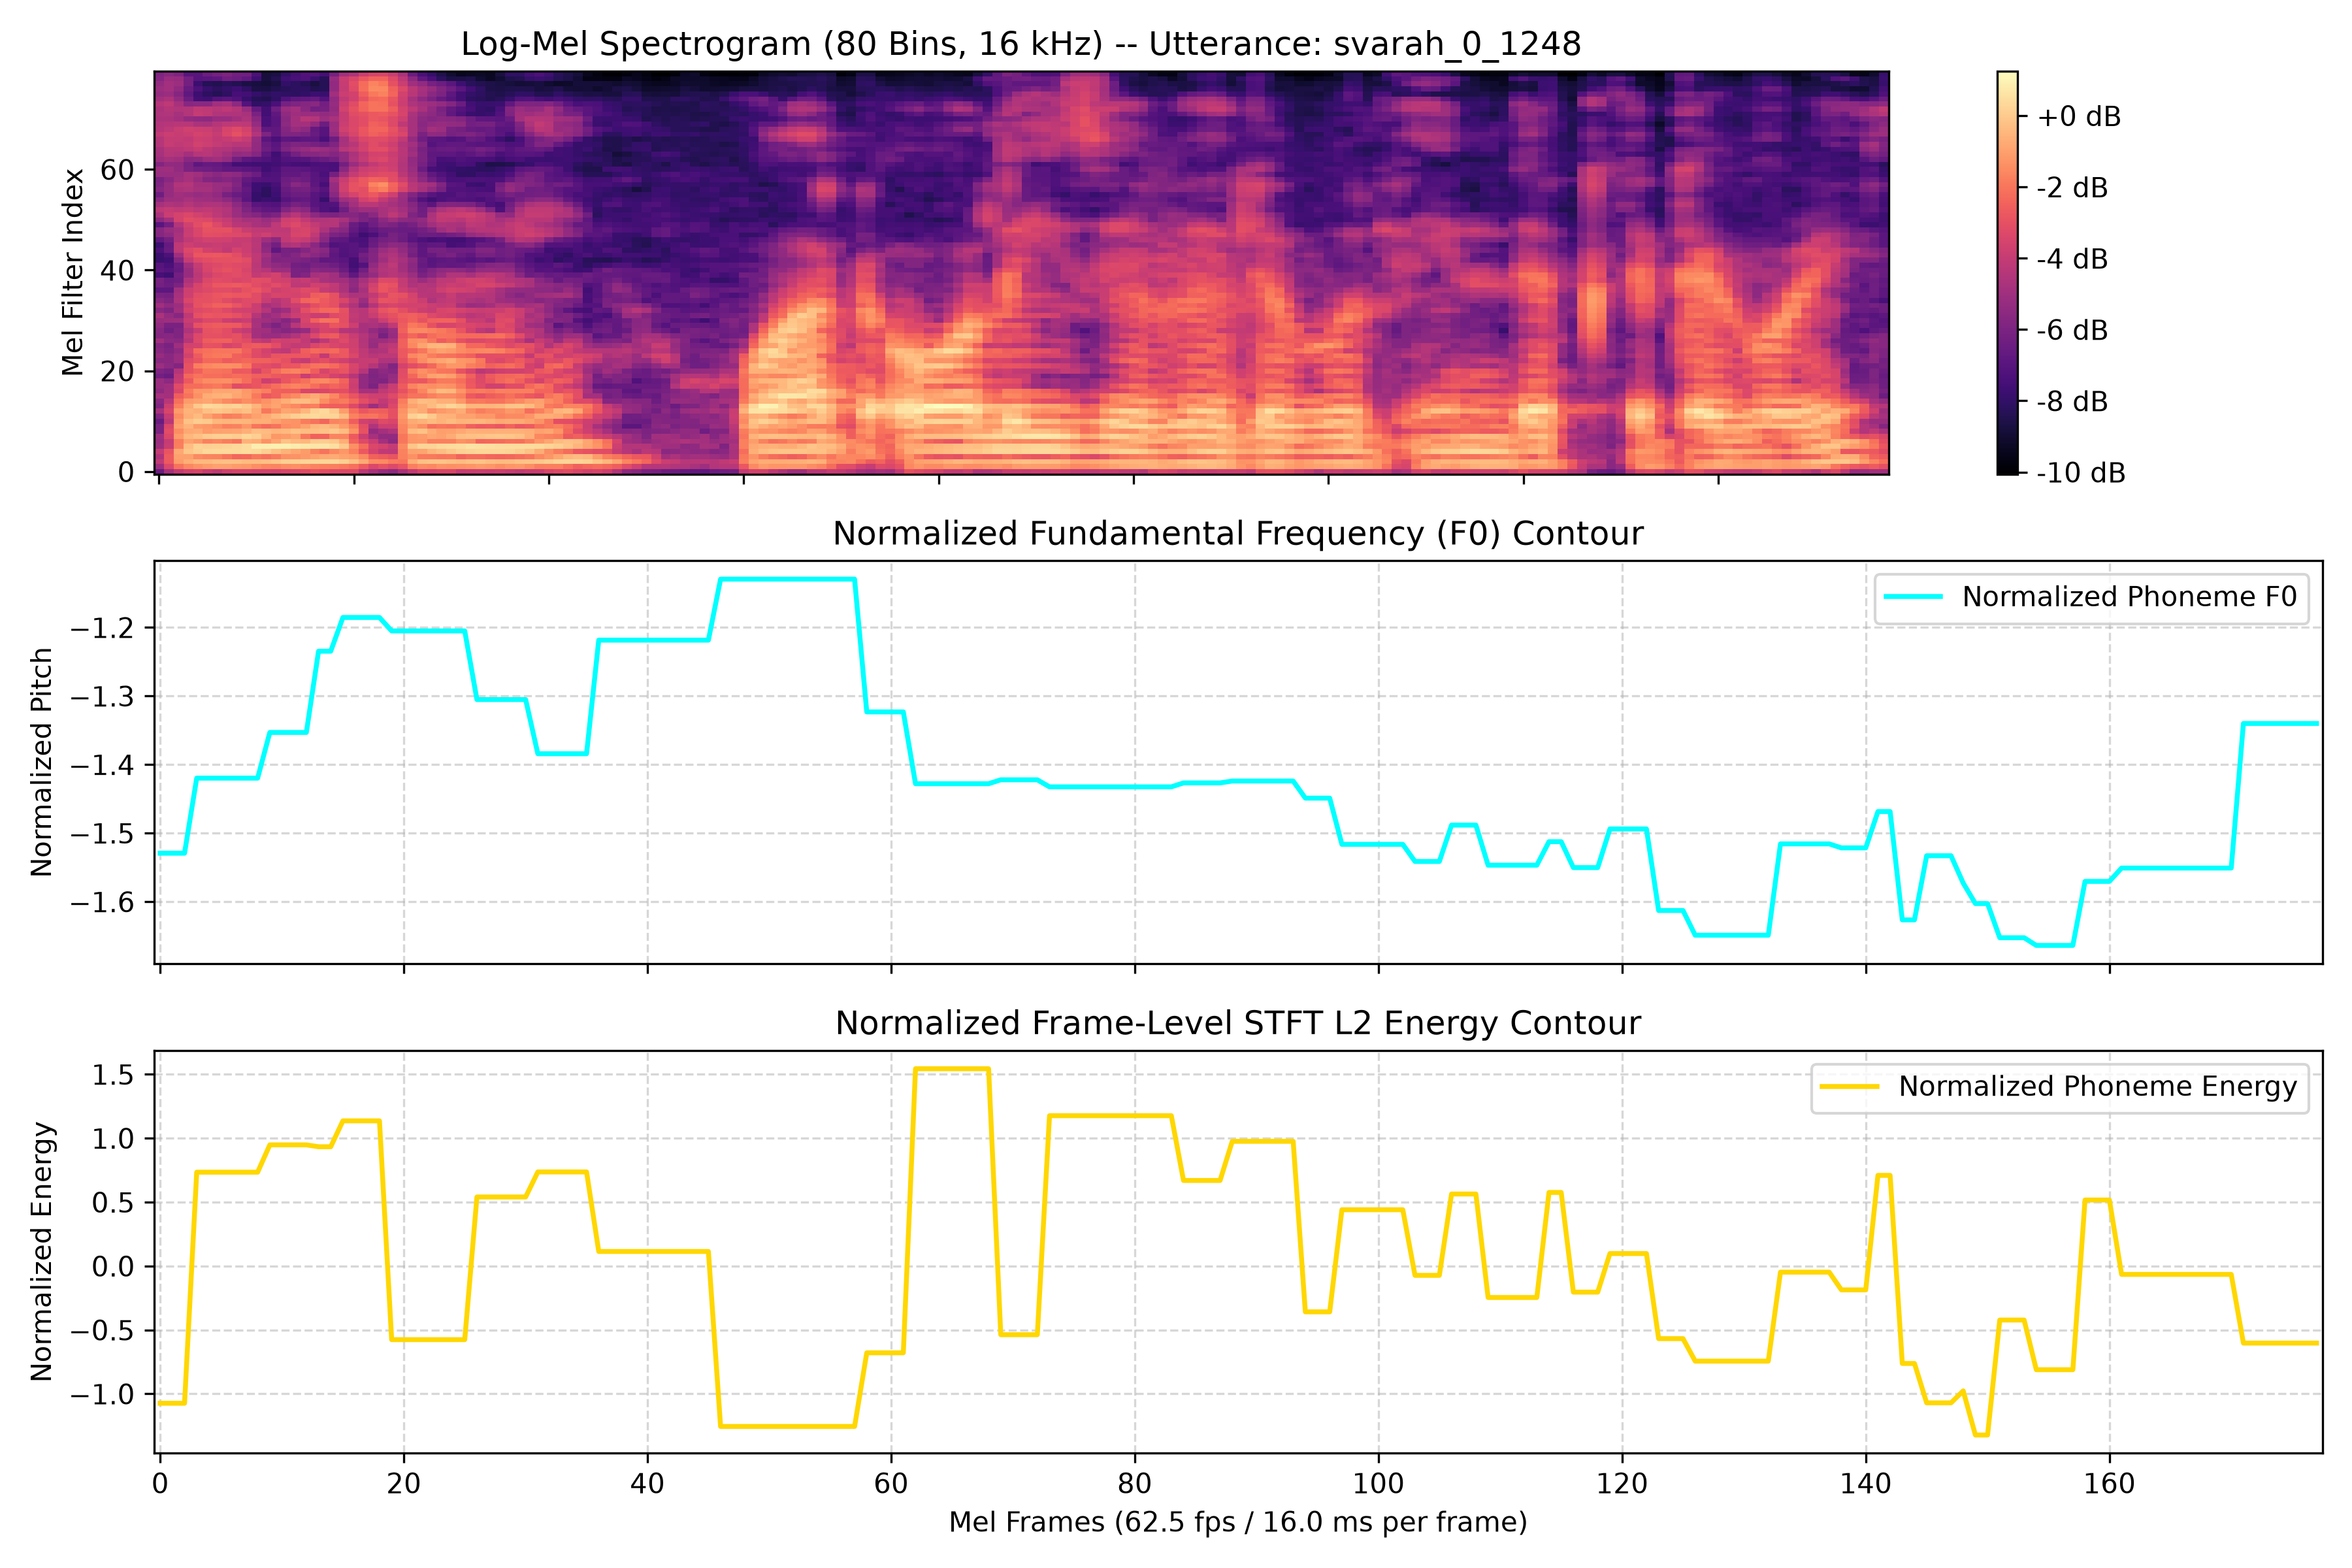
\includegraphics[width=\textwidth]{figures/diagnostic_features_example.png}
    \caption{Features of one utterance (\texttt{svarah\_0\_1248})}
\end{subfigure}
\hfill
\begin{subfigure}[b]{0.48\textwidth}
    \centering
    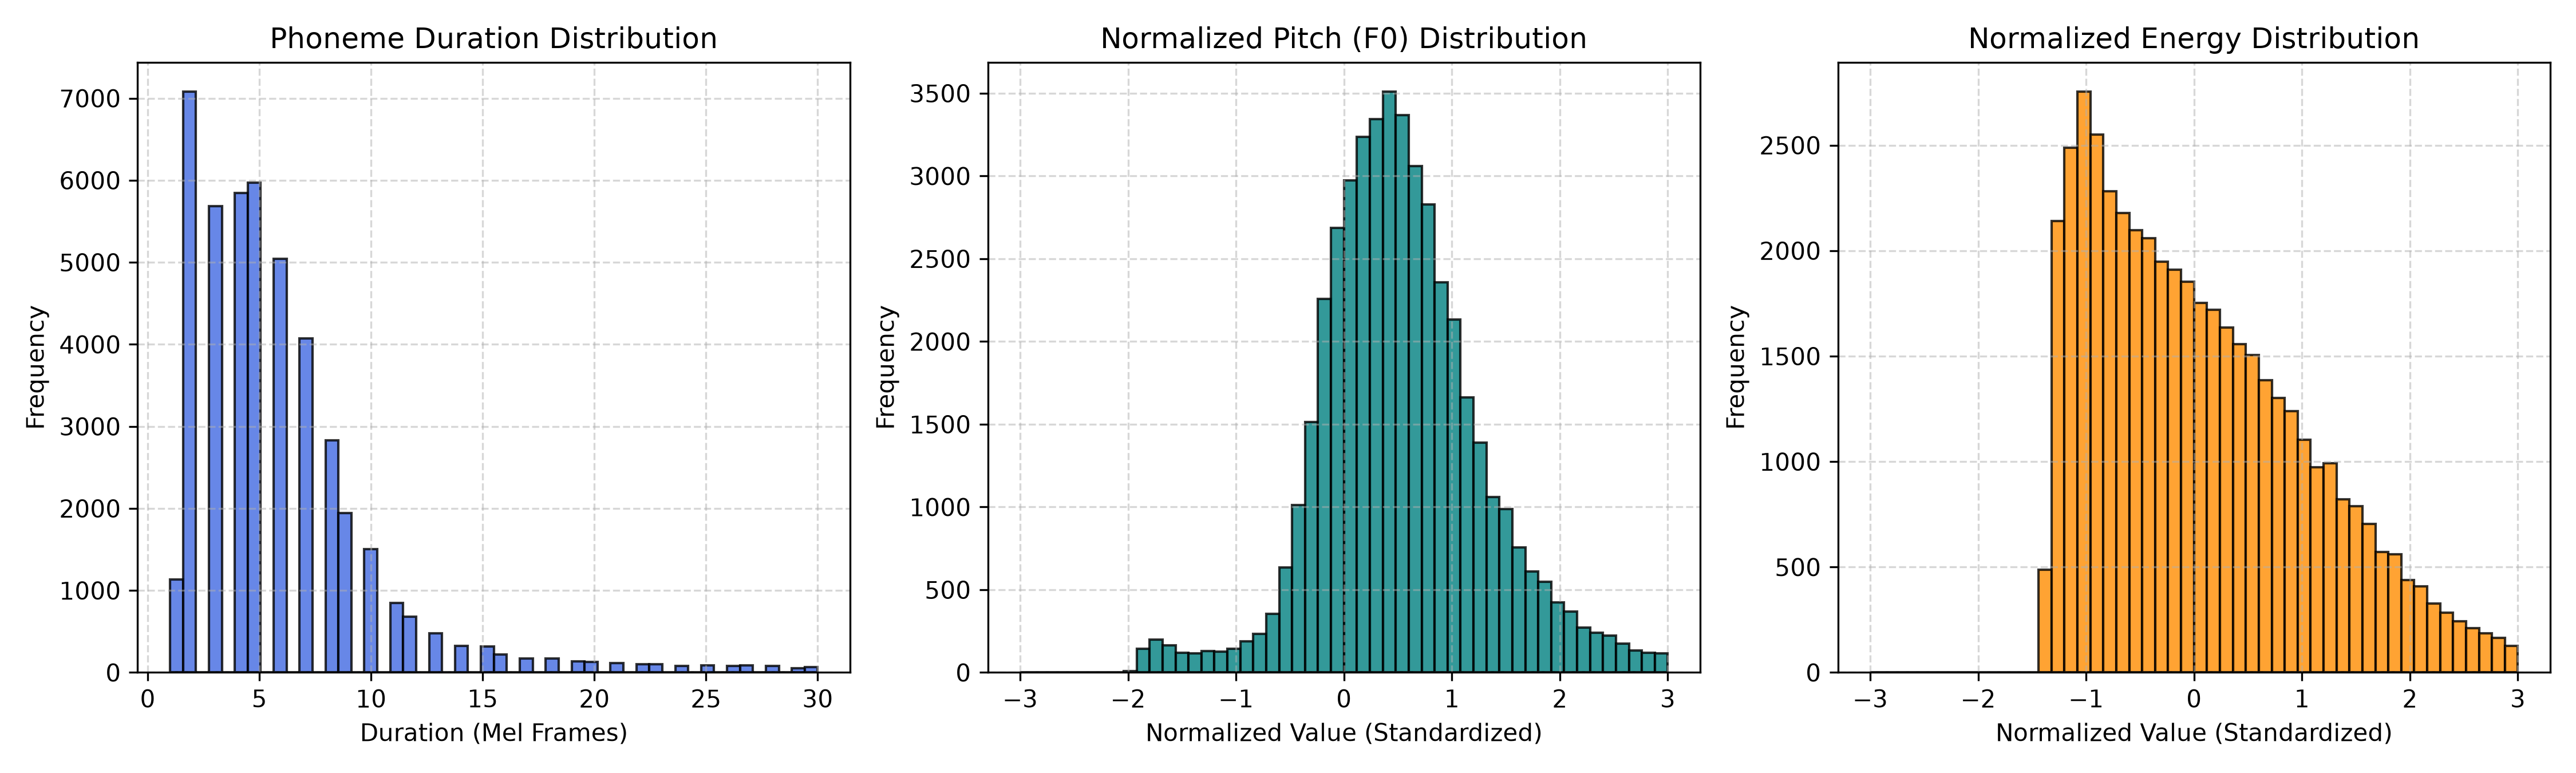
\includegraphics[width=\textwidth]{figures/diagnostic_feature_distributions.png}
    \caption{Training-set distributions used for normalisation}
\end{subfigure}
\caption{Feature check. Left: waveform, log-mel spectrogram, pitch contour and frame energy. Right: the distributions the z-score statistics come from.}
\label{fig:feature_diagnostics}
\end{figure}

% ------------------------------------------------------------------
% 7 MODEL
% ------------------------------------------------------------------
\section{Model Architecture}

\subsection{Overview}
FastSpeech 2 has three main parts: an FFT encoder, a variance adaptor and an FFT decoder. A convolutional post-net refines the output mel-spectrogram, and a neural vocoder turns it into audio (Figure~\ref{fig:architecture}).

\begin{figure}[H]
\centering
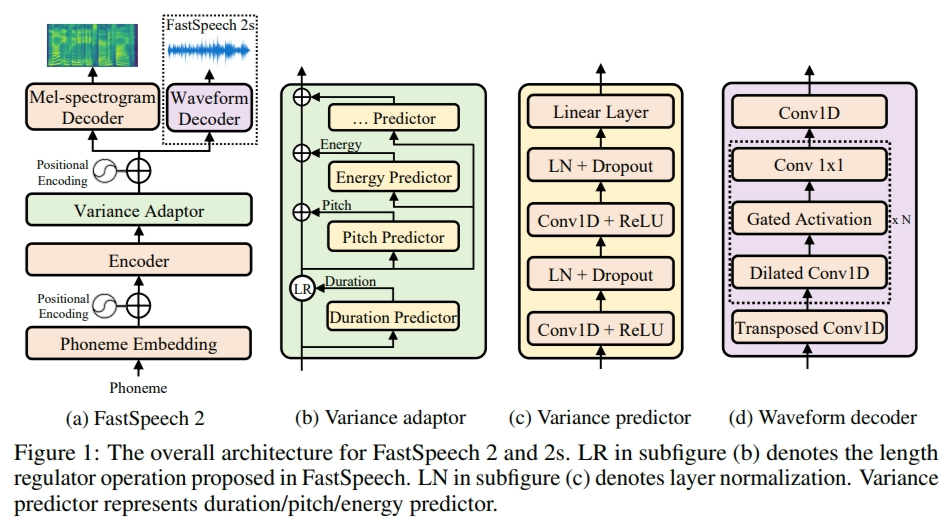
\includegraphics[width=0.8\textwidth]{figures/model_architecture.png}
\caption{The implemented architecture: FFT encoder, length regulator, variance predictors (duration, pitch, energy), FFT decoder, post-net and vocoder.}
\label{fig:architecture}
\end{figure}

\subsection{Encoder and Decoder}
The encoder consists of 4 FFT blocks, and the decoder consists of 6 FFT blocks. Each block has multi-head self-attention (2 heads, $d_{\text{model}}=256$) followed by a two-layer 1D convolutional feed-forward network (kernels 9 and 1, filter size 1024, ReLU, layer norm), with dropout 0.2.

\subsection{Variance Adaptor}
The variance adaptor connects the phoneme-length sequence to the longer mel-frame sequence and adds pitch and energy information:
\begin{enumerate}
    \item \textbf{Duration predictor:} two 1D conv layers (kernel 3, 256 filters, ReLU, layer norm, dropout 0.5) and a linear layer that outputs log-duration.
    \item \textbf{Length regulator:} repeats each phoneme's hidden vector as many times as its duration (ground truth during training, predicted at inference).
    \item \textbf{Pitch and energy predictors:} predict normalised $F_0$ and energy per phoneme. Their continuous scalar outputs are linearly quantized into 256 bins and projected into the encoder hidden dimension via \texttt{nn.Embedding} before being added to the expanded sequence.
\end{enumerate}

\subsection{Post-Net and Loss}
A 5-layer convolutional post-net predicts a residual that is added to the decoder's mel output. The total loss is
\begin{equation}
    \mathcal{L}_{\text{total}} = \mathcal{L}_{\text{mel}} + \mathcal{L}_{\text{postnet}} + \mathcal{L}_{\text{pitch}} + \mathcal{L}_{\text{energy}} + \mathcal{L}_{\text{duration}}
\end{equation}
Mel losses use L1 error. Duration, pitch and energy use mean squared error.

\subsection{HiFi-GAN Vocoder and the Sampling-Rate Problem}
I used the pre-trained universal HiFi-GAN vocoder~\cite{hifigan} (\texttt{generator\_universal.pth.tar}). It was trained on 22{,}050 Hz audio (hop 256), but my acoustic models use 16{,}000 Hz (hop 256). If the vocoder output is simply saved at 16 kHz without resampling, every sample is played back too slowly, so pitch and formants drop by
\begin{equation}
    \frac{16{,}000}{22{,}050} \approx 0.7256 \quad (\approx -5.5\text{ semitones})
\end{equation}
and speech sounds deep and muffled.

To resolve this, I added a polyphase sinc resampling bridge in \texttt{utils/model.py}. The vocoder runs at its native 22{,}050 Hz and its output is resampled to 16 kHz before being saved. While this successfully restores the correct pitch and harmonic frequencies, decimating the samples by a factor of $16{,}000 / 22{,}050 \approx 0.7256$ contracts the effective duration per frame from 16.0 ms to 11.6 ms. This explains why the baseline model ($d_{\text{control}}=1.0$) generated speech about 1.38$\times$ faster than natural rate. Calibrating the duration control parameter during inference ($d_{\text{control}}=1.378$ for English, $1.40$ for Telugu) directly compensates for this ratio and restores natural pacing without retraining.

% ------------------------------------------------------------------
% 8 TRAINING
% ------------------------------------------------------------------
\section{Training}

\subsection{Setup}
Both models were trained on Kaggle with two NVIDIA Tesla T4 GPUs (16 GB each, \texttt{DataParallel}). Table~\ref{tab:hyperparams} lists the settings, which were identical for both languages.

\begin{table}[H]
\centering
\caption{Training configuration (same for English and Telugu unless noted).}
\label{tab:hyperparams}
\small
\begin{tabularx}{\textwidth}{lX}
\toprule
\textbf{Setting} & \textbf{Value} \\
\midrule
Batch size & 16 (8 per GPU) \\
Total steps & 100{,}000 \\
Training audio & English: 4.98 h (3{,}419 utt.); Telugu: 4.18 h (2{,}248 utt.) \\
Validation audio & English: 1.09 h (746 utt.); Telugu: 0.82 h (445 utt.) \\
Optimiser & AdamW ($\beta_1=0.9$, $\beta_2=0.98$, $\epsilon=10^{-9}$) \\
Learning-rate schedule & Noam, 4{,}000 warm-up steps \\
Peak learning rate & $\approx 9.9\times10^{-4}$ (Noam formula, $d_{\text{model}}=256$) \\
Gradient clipping & $\|g\|_2 \le 1.0$ \\
Mixed precision & PyTorch AMP (FP16) \\
Model size & 4 encoder / 6 decoder FFT blocks, $d_{\text{model}}=256$, 2 heads, filter size 1024 \\
Validation & every 1{,}000 steps; top-3 checkpoints kept \\
\bottomrule
\end{tabularx}
\end{table}

Because of Kaggle's 12-hour session limit, each model was trained in two runs. The first run ended at step 53{,}000 for English and 56{,}000 for Telugu. The second run resumed from the last saved checkpoint and continued to step 100{,}000.

\subsection{Loss Curves}
Figures~\ref{fig:loss_english} and~\ref{fig:loss_telugu} show training and validation loss over the full 100{,}000 steps.

\begin{figure}[H]
\centering
\begin{subfigure}{0.48\textwidth}
    \centering
    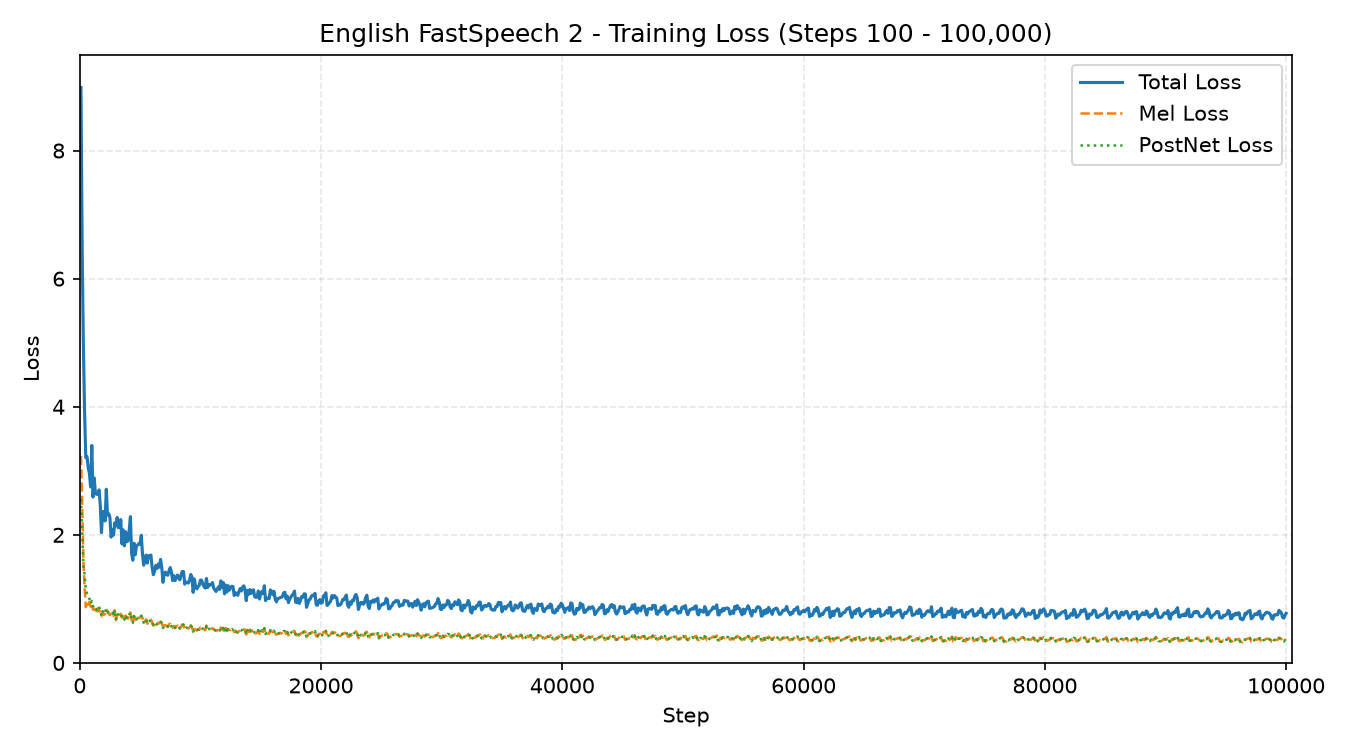
\includegraphics[width=\textwidth]{figures/english_training_loss.png}
    \caption{Training loss}
\end{subfigure}
\hfill
\begin{subfigure}{0.48\textwidth}
    \centering
    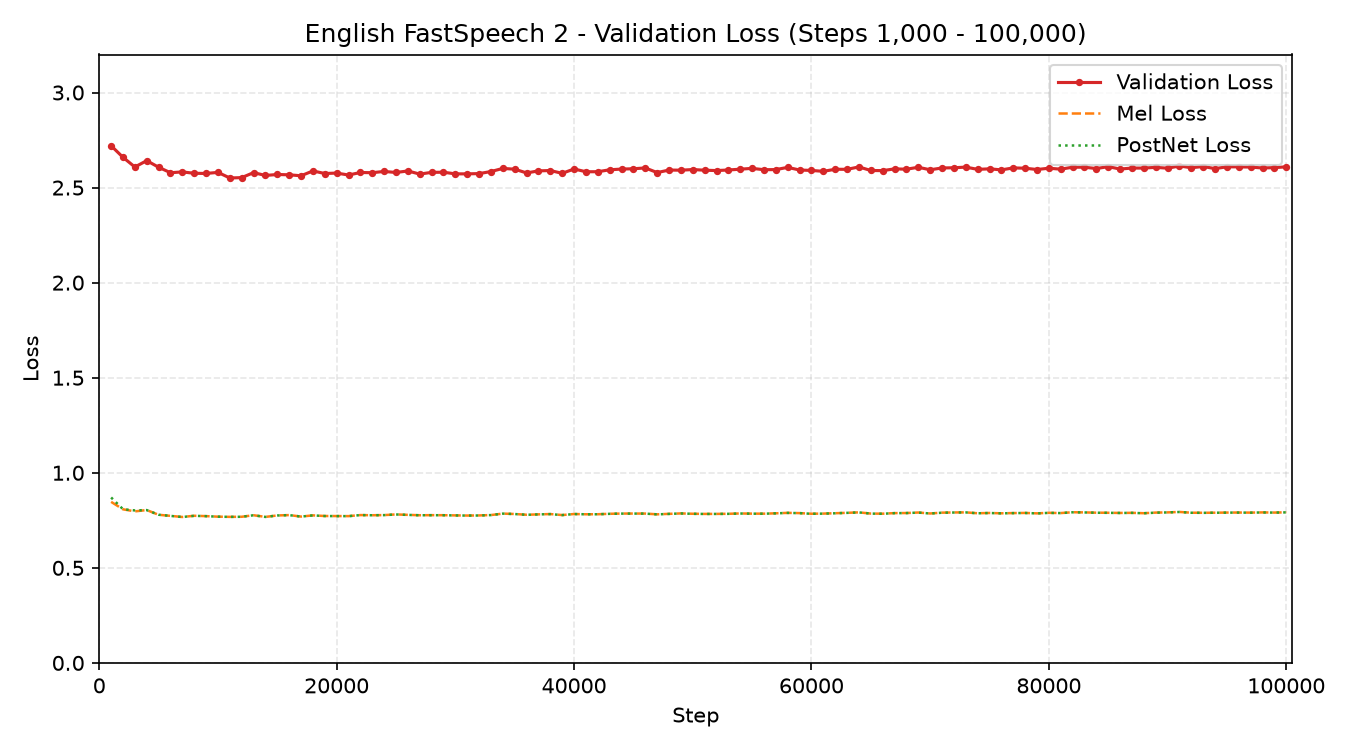
\includegraphics[width=\textwidth]{figures/english_validation_loss.png}
    \caption{Validation loss}
\end{subfigure}
\caption{English training and validation loss.}
\label{fig:loss_english}
\end{figure}

\begin{figure}[H]
\centering
\begin{subfigure}{0.48\textwidth}
    \centering
    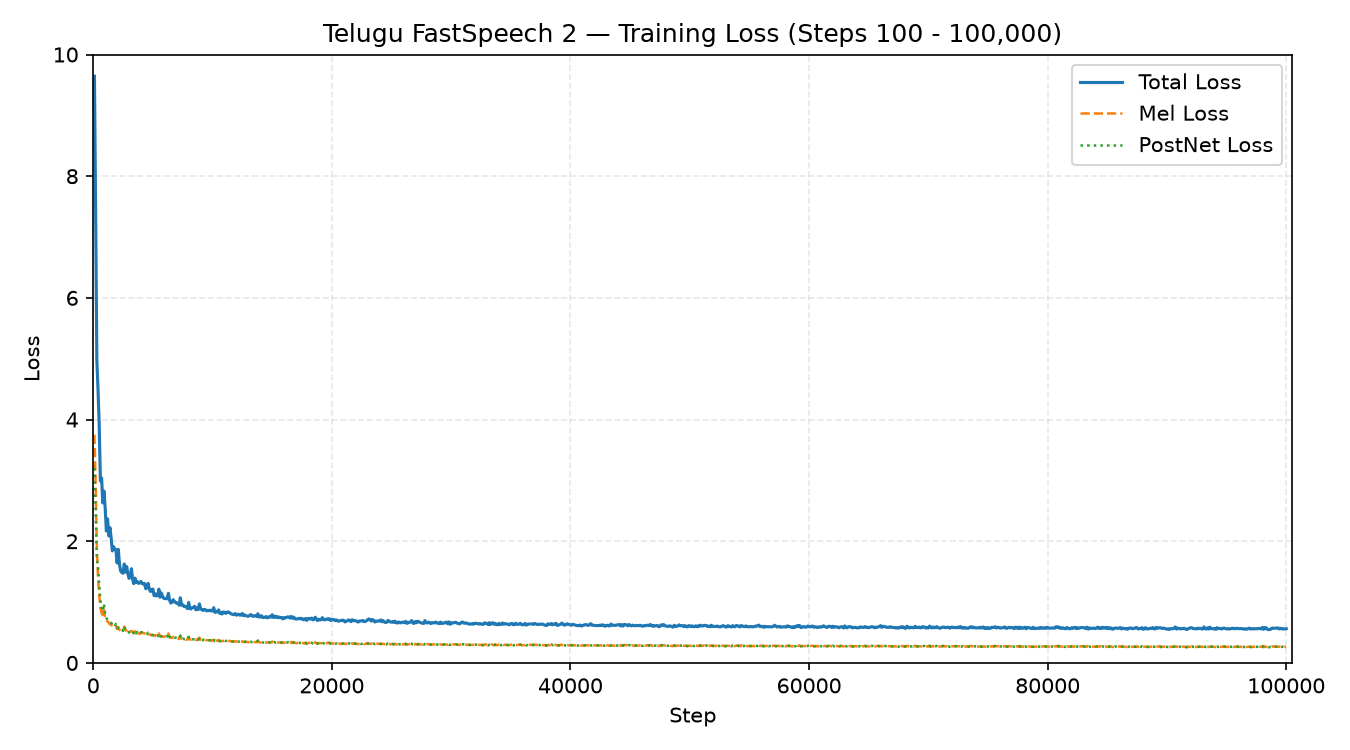
\includegraphics[width=\textwidth]{figures/telugu_training_loss.png}
    \caption{Training loss}
\end{subfigure}
\hfill
\begin{subfigure}{0.48\textwidth}
    \centering
    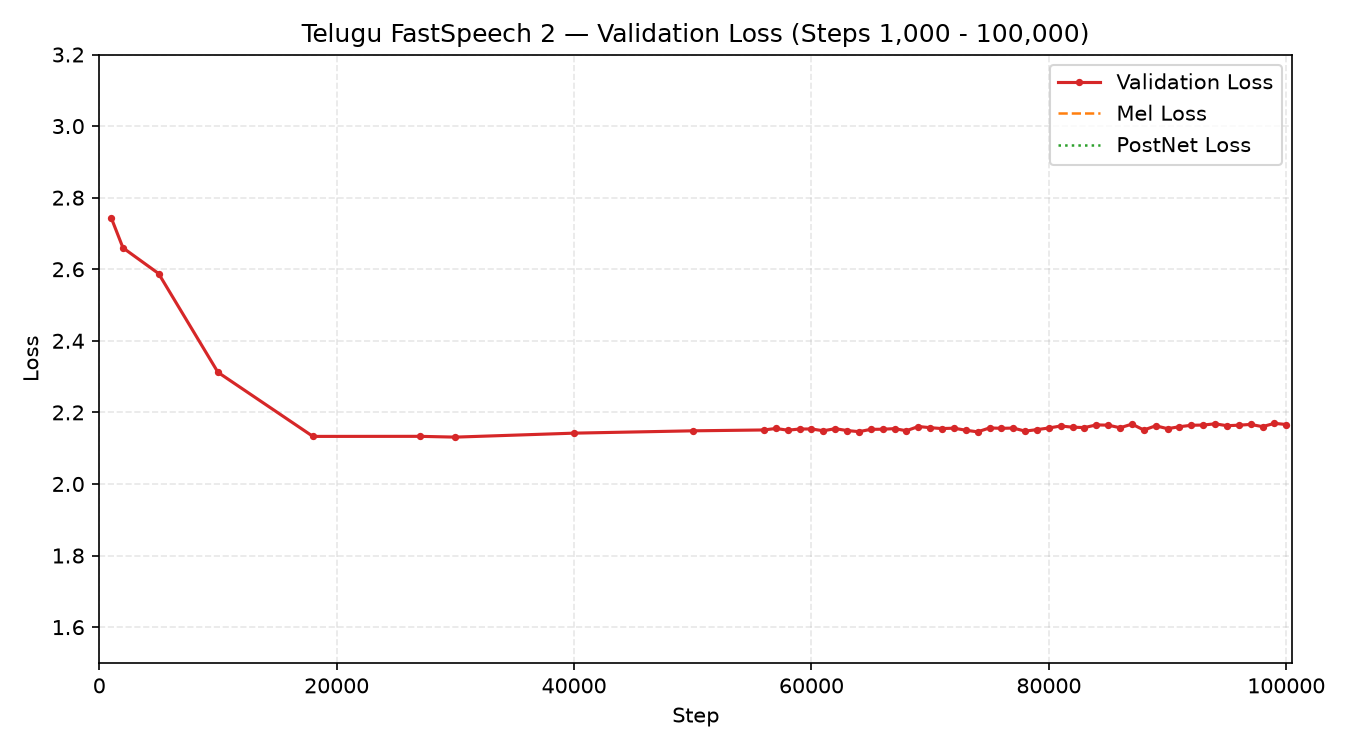
\includegraphics[width=\textwidth]{figures/telugu_validation_loss.png}
    \caption{Validation loss}
\end{subfigure}
\caption{Telugu training and validation loss.}
\label{fig:loss_telugu}
\end{figure}

\subsection{Convergence, Overfitting and Checkpoint Choice}\label{sec:overfit}
The training loss dropped steeply during the first 20{,}000 steps and then declined slowly for both models. The validation loss behaved differently, as Table~\ref{tab:ckpt} shows.

\begin{table}[H]
\centering
\caption{Key checkpoints. Validation loss is lowest early, while training loss is still high.}
\label{tab:ckpt}
\small
\begin{tabular}{llccc}
\toprule
\textbf{Language} & \textbf{Checkpoint} & \textbf{Step} & \textbf{Train loss} & \textbf{Val loss} \\
\midrule
English & Lowest validation loss & 11{,}000 & 2.5887 & 2.5505 \\
English & Used for synthesis & 61{,}000 & 0.8415 & 2.5855 \\
Telugu & Lowest validation loss (run 1) & 30{,}000 & -- & 2.1309 \\
Telugu & Used for synthesis & 74{,}000 & 0.6412 & 2.1457 \\
\bottomrule
\end{tabular}
\end{table}

What this shows:
\begin{itemize}
    \item \textbf{Overfitting.} At the chosen checkpoints the validation loss is about three times the training loss (2.59 vs 0.84 for English, 2.15 vs 0.64 for Telugu). It also never got meaningfully better after its early minimum. With only 4--5 hours of training data the models memorise the training set faster than they improve on new sentences.
    \item \textbf{Why I did not use the lowest-validation checkpoints.} At step 11{,}000 (English) the training loss was still 2.59, and when I listened to that checkpoint the speech was muffled and consonants were unclear. A blurry, averaged mel-spectrogram can still give a low L1 loss. The step-61{,}000 model had sharper formants and clearer consonants, so I selected it by listening. I did the same for Telugu (step 74{,}000). The file \texttt{best\_model.pth} therefore points to these hand-picked checkpoints, not to the lowest validation loss.
    \item \textbf{Stability.} The training runs proceeded stably without loss divergence. Gradient clipping ($\|g\|_2 \le 1.0$) and FP16 mixed precision were used throughout. The restart between the two runs was seamless with full AdamW state restoration, showing no discontinuities in the loss progression.
    \item \textbf{English vs Telugu.} Telugu has the lower validation loss (2.15 vs 2.59). This should not be read as ``Telugu is better'' because the two losses use different symbol sets, different feature statistics and different data. A plausible reason is that the Telugu data comes from two studio speakers while Svarah has 104 speakers with very different recording conditions, so there is simply less variation to predict.
\end{itemize}

% ------------------------------------------------------------------
% 9 RESULTS
% ------------------------------------------------------------------
\section{Synthesis Results}

\subsection{How the Test Sentences Were Generated}
Each test sentence was converted to symbols, passed through the model (encoder, variance adaptor, decoder, post-net), and the mel output was converted to audio by HiFi-GAN and resampled to 16 kHz. All English test sentences were synthesized using Speaker ID 27 (\texttt{spk\_029}), and all Telugu test sentences were synthesized using Speaker ID 0 (\texttt{telugufemale}), ensuring consistency within each language.
No formal listening test (such as MOS) was run. My observations come from informal listening and from the measurements read off the variance-adaptor plots. The sentence text was given to the model exactly as printed in the assignment, except for the whitespace handling described under E3 and T3.

\subsection{Measurements for All Ten Sentences}
\begin{table}[H]
\centering
\caption{Acoustic measurements of the generated test sentences. The five English sentences add up to about 15.8 s of audio and the five Telugu sentences to about 12.6 s under baseline inference.}
\label{tab:eval_metrics}
\scriptsize
\begin{tabularx}{\textwidth}{llXrrrrrr}
\toprule
\textbf{ID} & \textbf{Lang} & \textbf{Text (shortened)} & \textbf{Dur (s)} & \textbf{Frames} & \textbf{Mean $F_0$} & \textbf{$F_0$ range} & \textbf{Energy} & \textbf{Rate} \\
\midrule
E1 & Eng & The antidisestablishmentarianism movement gained\ldots & 4.01 & 345 & 212.1 Hz & 168--248 Hz & 64.5 dB & 4.49 syl/s \\
E2a & Eng & The orchestra's conduct during the ceremony\ldots & 2.68 & 231 & 212.8 Hz & 184--238 Hz & 52.0 dB & 4.85 syl/s \\
E2b & Eng & The researchers will conduct an experiment\ldots & 2.87 & 247 & 207.8 Hz & 172--242 Hz & 55.5 dB & 4.88 syl/s \\
E3 & Eng & The rhyth m of the orchestra changed unexpectedly. & 1.75 & 151 & 207.9 Hz & 181--234 Hz & 60.5 dB & 5.13 syl/s \\
E4 & Eng & The meeting will start at 10:45 AM on 12 November 2026\ldots & 4.46 & 384 & 213.2 Hz & 182--246 Hz & 60.5 dB & 4.71 syl/s \\
\midrule
T1 & Tel & \texttelugu{న్యూరోఫార్మకోలాజికల్ పరిశోధనలో\ldots} & 3.37 & 290 & 207.6 Hz & 154--258 Hz & 56.0 dB & 5.35 syl/s \\
T2a & Tel & \texttelugu{తాడుపై అతని పట్టు చాలా బలంగా ఉంది.} & 1.57 & 135 & 219.0 Hz & 162--274 Hz & 65.7 dB & 6.38 syl/s \\
T2b & Tel & \texttelugu{ఆమె పట్టు చీరను ధరించి వేడుకకు వచ్చింది.} & 1.67 & 144 & 201.9 Hz & 158--246 Hz & 57.1 dB & 6.58 syl/s \\
T3 & Tel & \texttelugu{పులి అడ  విలో నిశ్శబ్దంగా నడిచింది.} & 1.54 & 133 & 224.8 Hz & 160--282 Hz & 71.9 dB & 5.83 syl/s \\
T4 & Tel & \texttelugu{ఈ సమావేశం 2026 నవంబర్ 12వ తేదీ\ldots} & 4.40 & 379 & 196.8 Hz & 152--241 Hz & 56.5 dB & 6.59 syl/s \\
\bottomrule
\end{tabularx}
\end{table}

A few general patterns are visible in the table. Telugu is spoken faster in syllables per second (5.4--6.6 vs 4.5--5.1), which fits a language where each akshara has a fairly even length. Mean pitch is 197--225 Hz for all sentences, reflecting the female reference voices selected for synthesis. Overall the speech is clear and intelligible.

\subsection{English Test Sentences}

\subsubsection{E1: A Very Long Word}
\textit{``The antidisestablishmentarianism movement gained considerable momentum during the parliamentary proceedings.''}

The word \textit{antidisestablishmentarianism} is 28 letters long and becomes 27 phoneme tokens. The duration predictor gave each phoneme about 45.5 ms, so no syllable was dropped or merged. The pitch falls gradually over the sentence, with a peak of 234.1 Hz on \textit{momentum} and a final value of 186.2 Hz. I heard slightly weak high-frequency detail around the \texttt{/s ʈ/} sequence, which is typical of this kind of model.

\begin{figure}[H]
\centering
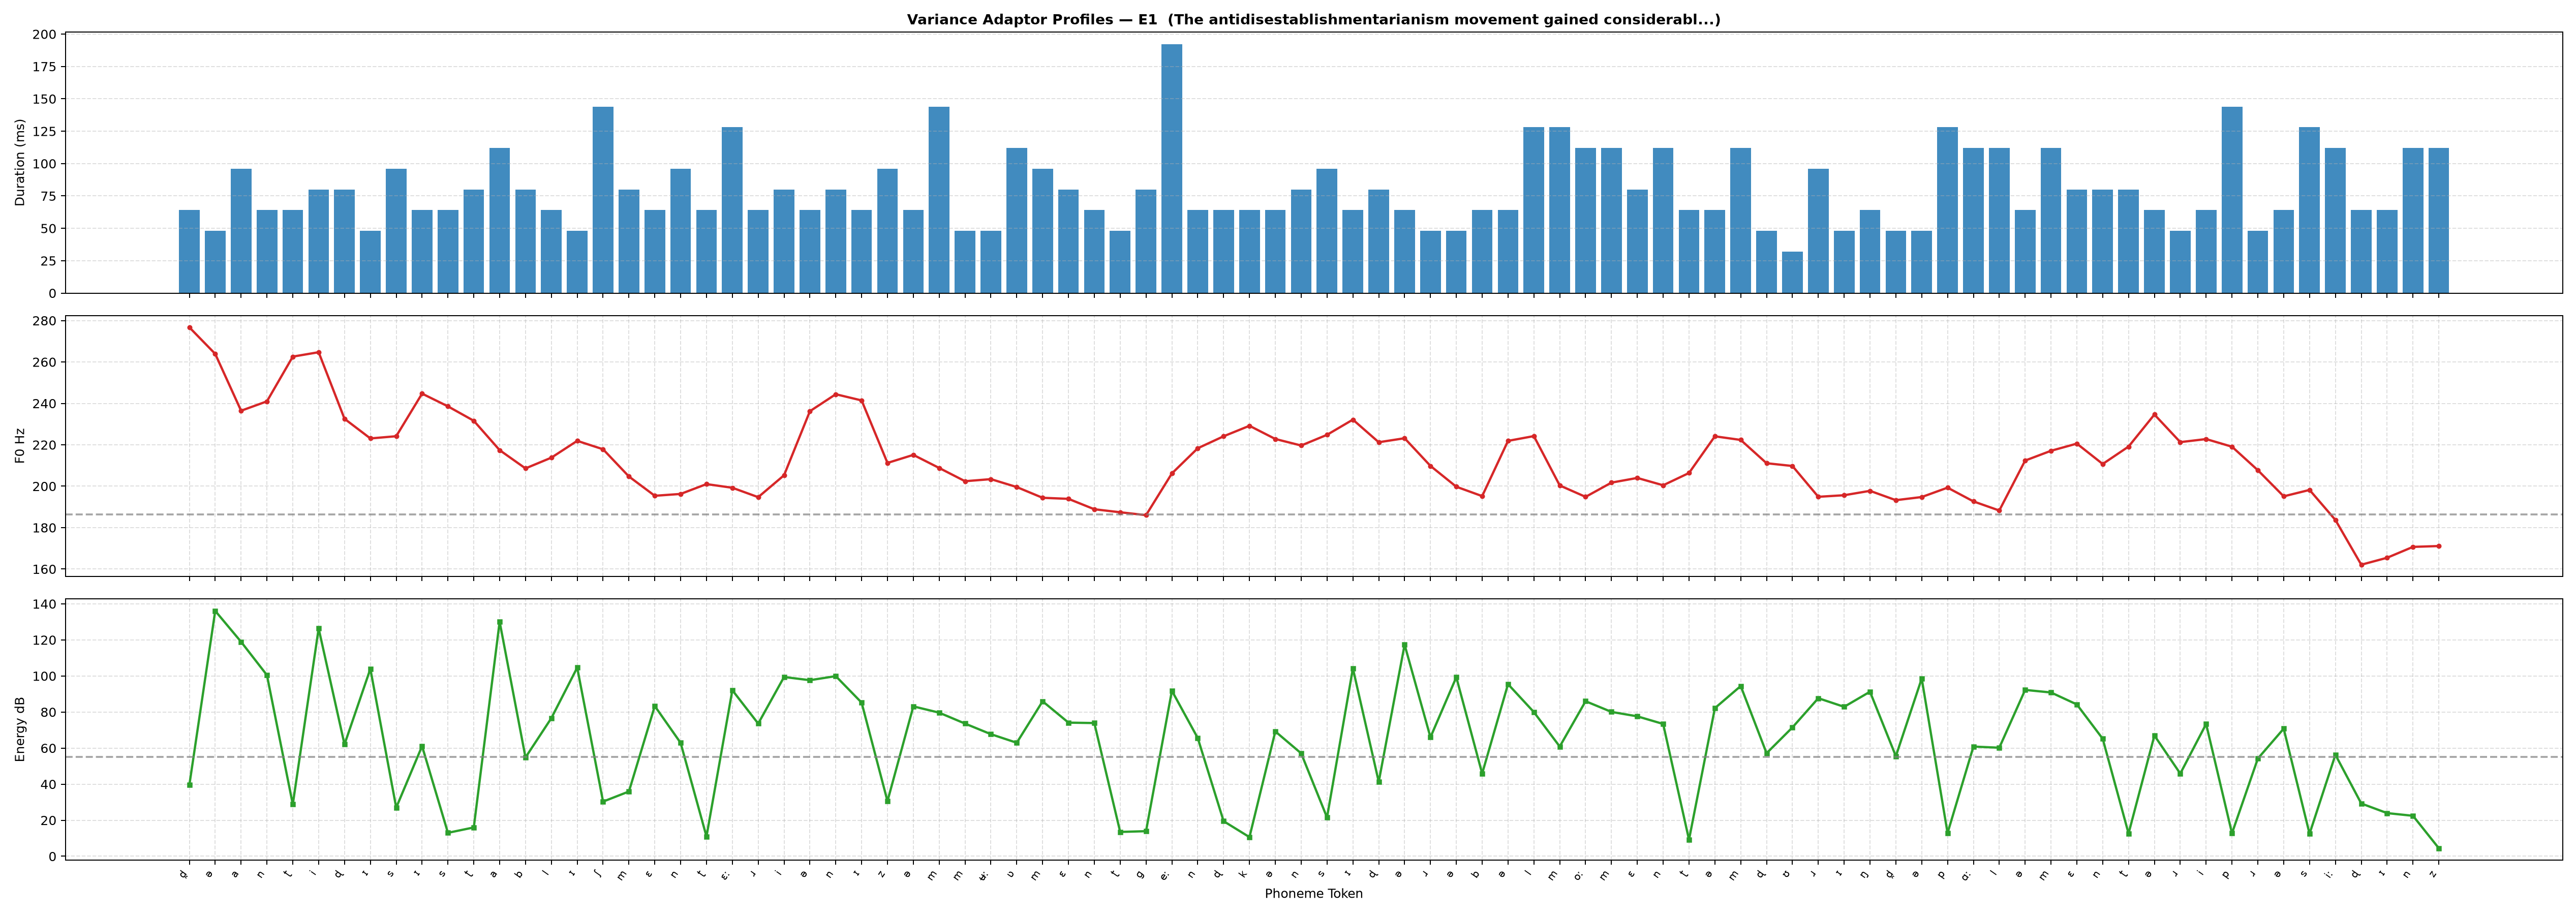
\includegraphics[width=\textwidth]{figures/E1_variance_profiles.png}
\caption{Predicted duration, pitch and energy for E1.}
\label{fig:e1}
\end{figure}

\subsubsection{E2: The Heteronym \textit{conduct}}
\textbf{E2a (noun):} \textit{``The orchestra's conduct during the ceremony was praised by the audience.''}\\
\textbf{E2b (verb):} \textit{``The researchers will conduct an experiment to evaluate the proposed method.''}

This pair checks whether the model gets the stress right. As a noun, \textit{conduct} is stressed on the first syllable, and the plots agree: the first syllable \texttt{/k ɒ n/} is long (64.0 ms) and loud (56.8 dB). As a verb the stress moves to the second syllable. The first vowel reduces to a schwa \texttt{/k ə n/} (32.0 ms, 48.2 dB) and the second syllable \texttt{/ɖ ə k ʈ/} gets 57.9 dB, which is 9.7 dB more than the first. This works because the pronunciations are determined by the phoneme sequence the front-end produced. The model itself does not decide which reading to use.

\begin{figure}[H]
\centering
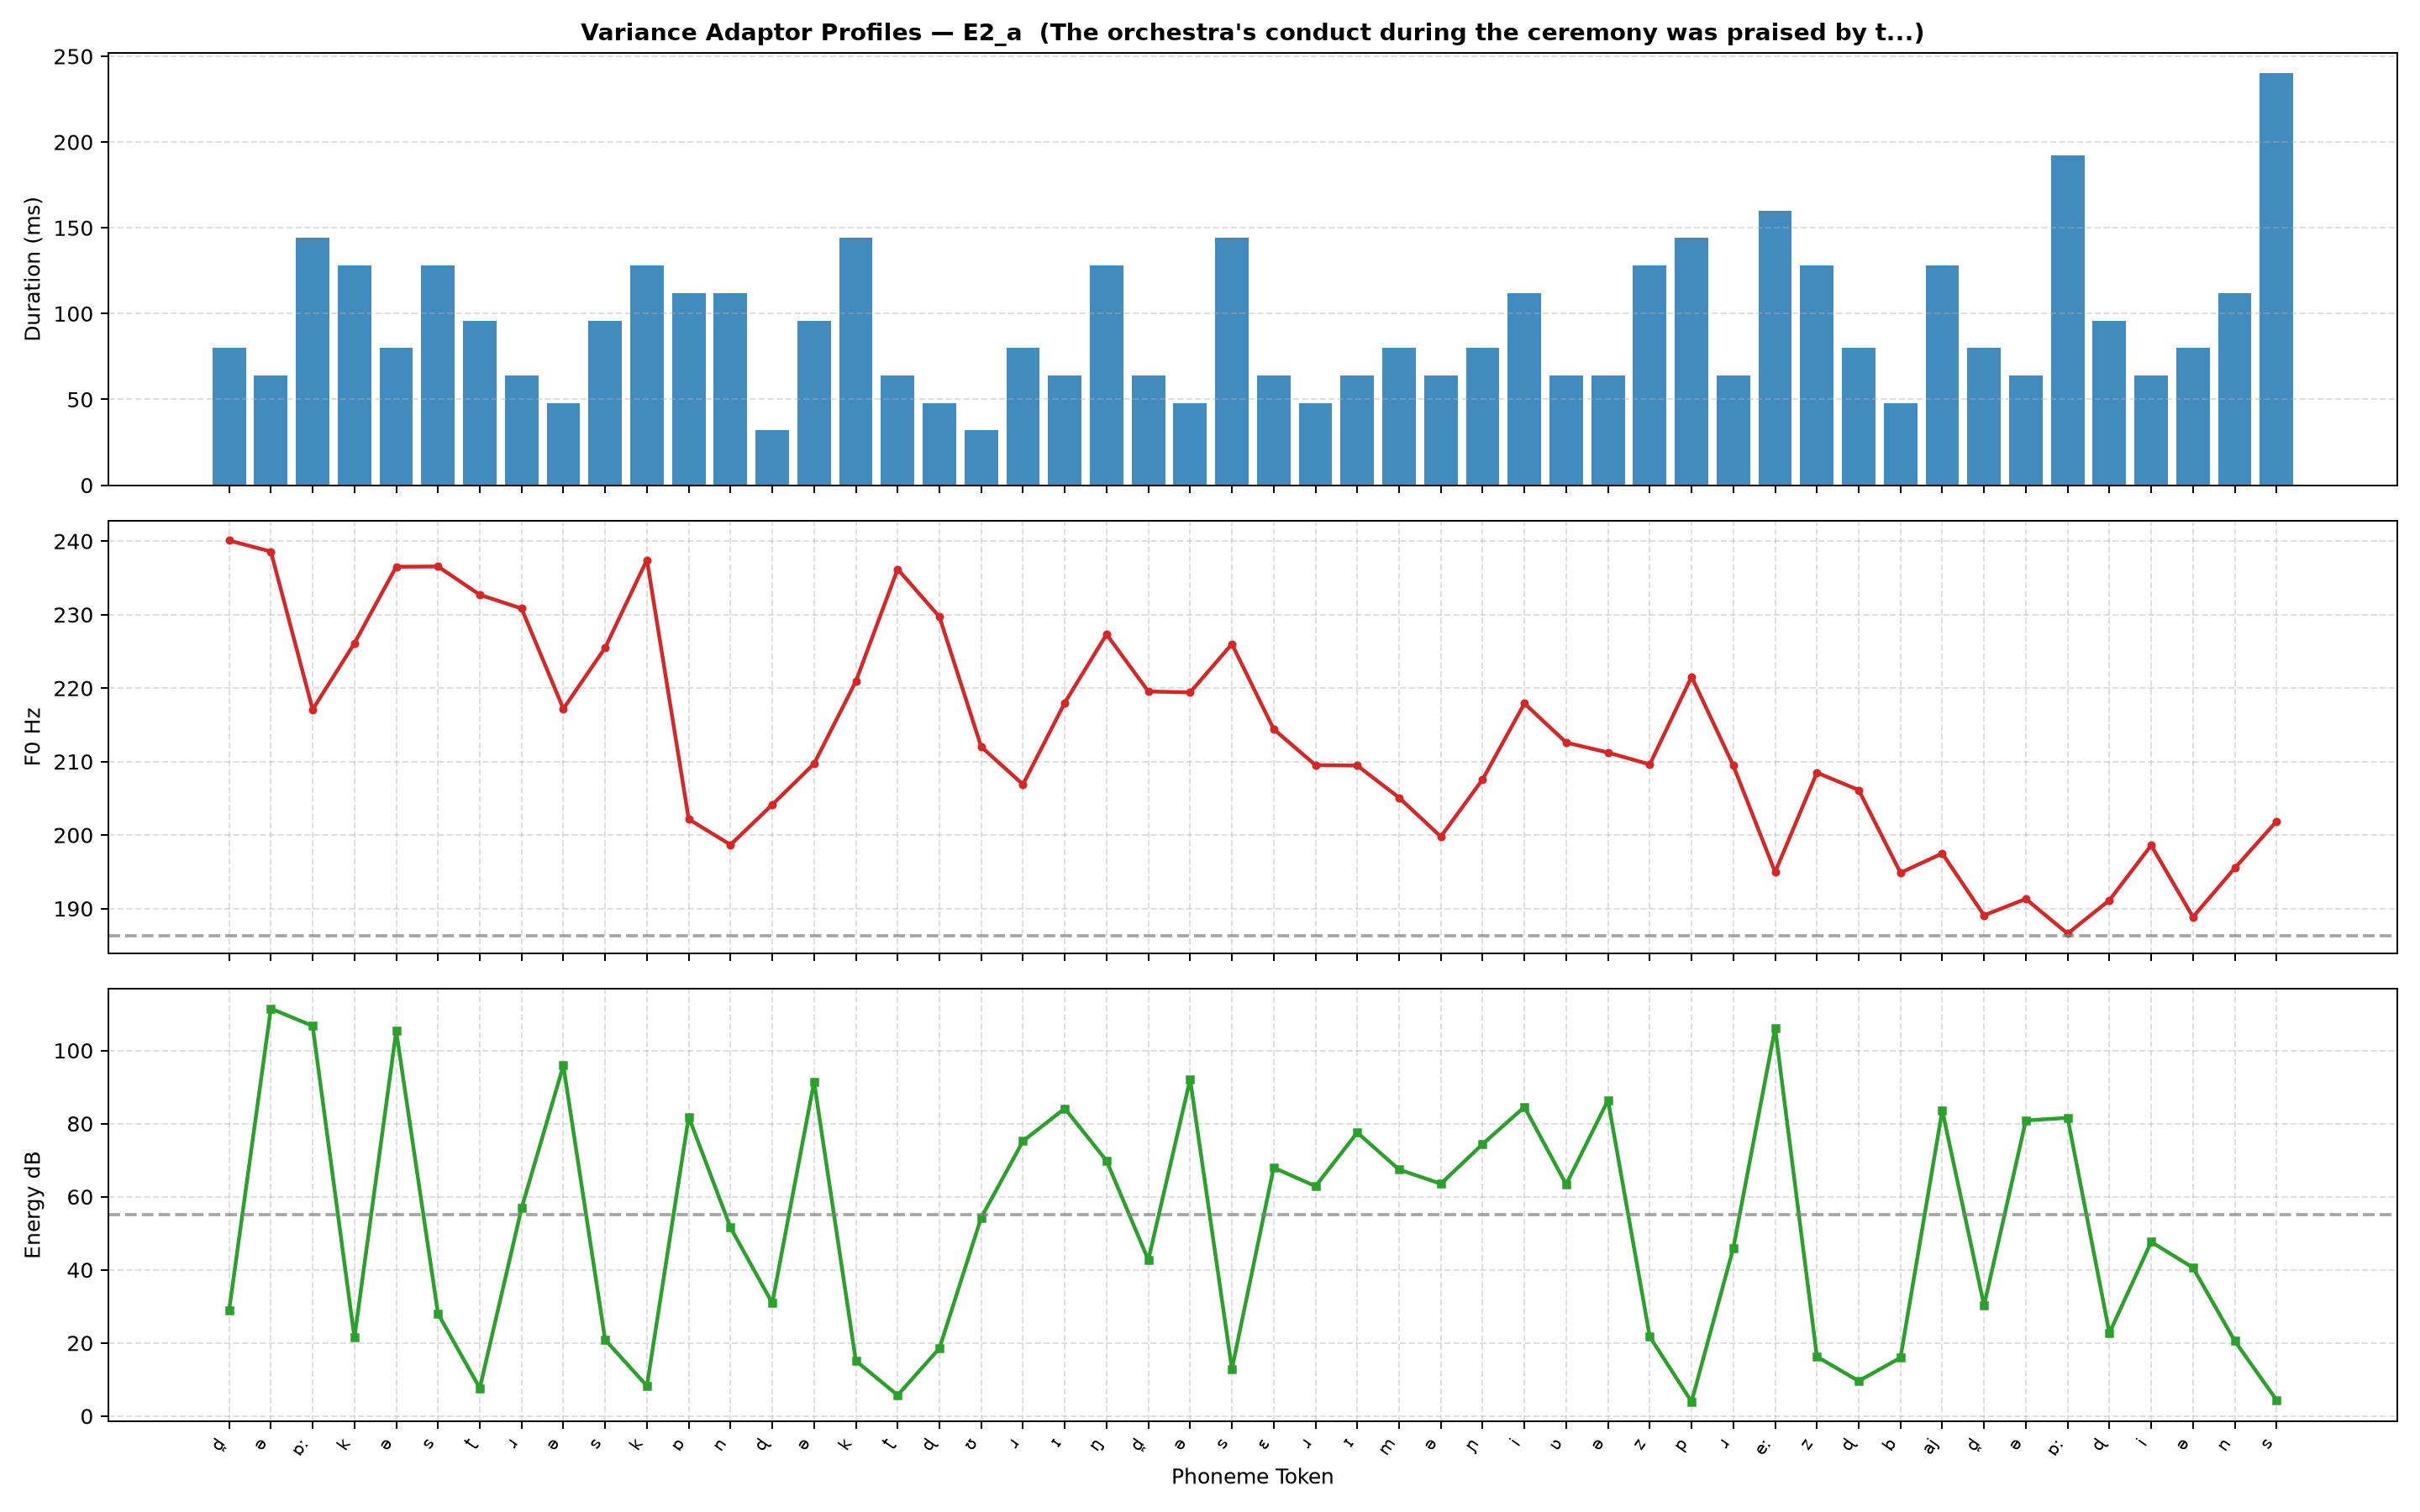
\includegraphics[width=\textwidth]{figures/E2a_variance_profiles.png}
\caption{Predicted duration, pitch and energy for E2a (noun \textit{conduct}).}
\label{fig:e2a}
\end{figure}

\begin{figure}[H]
\centering
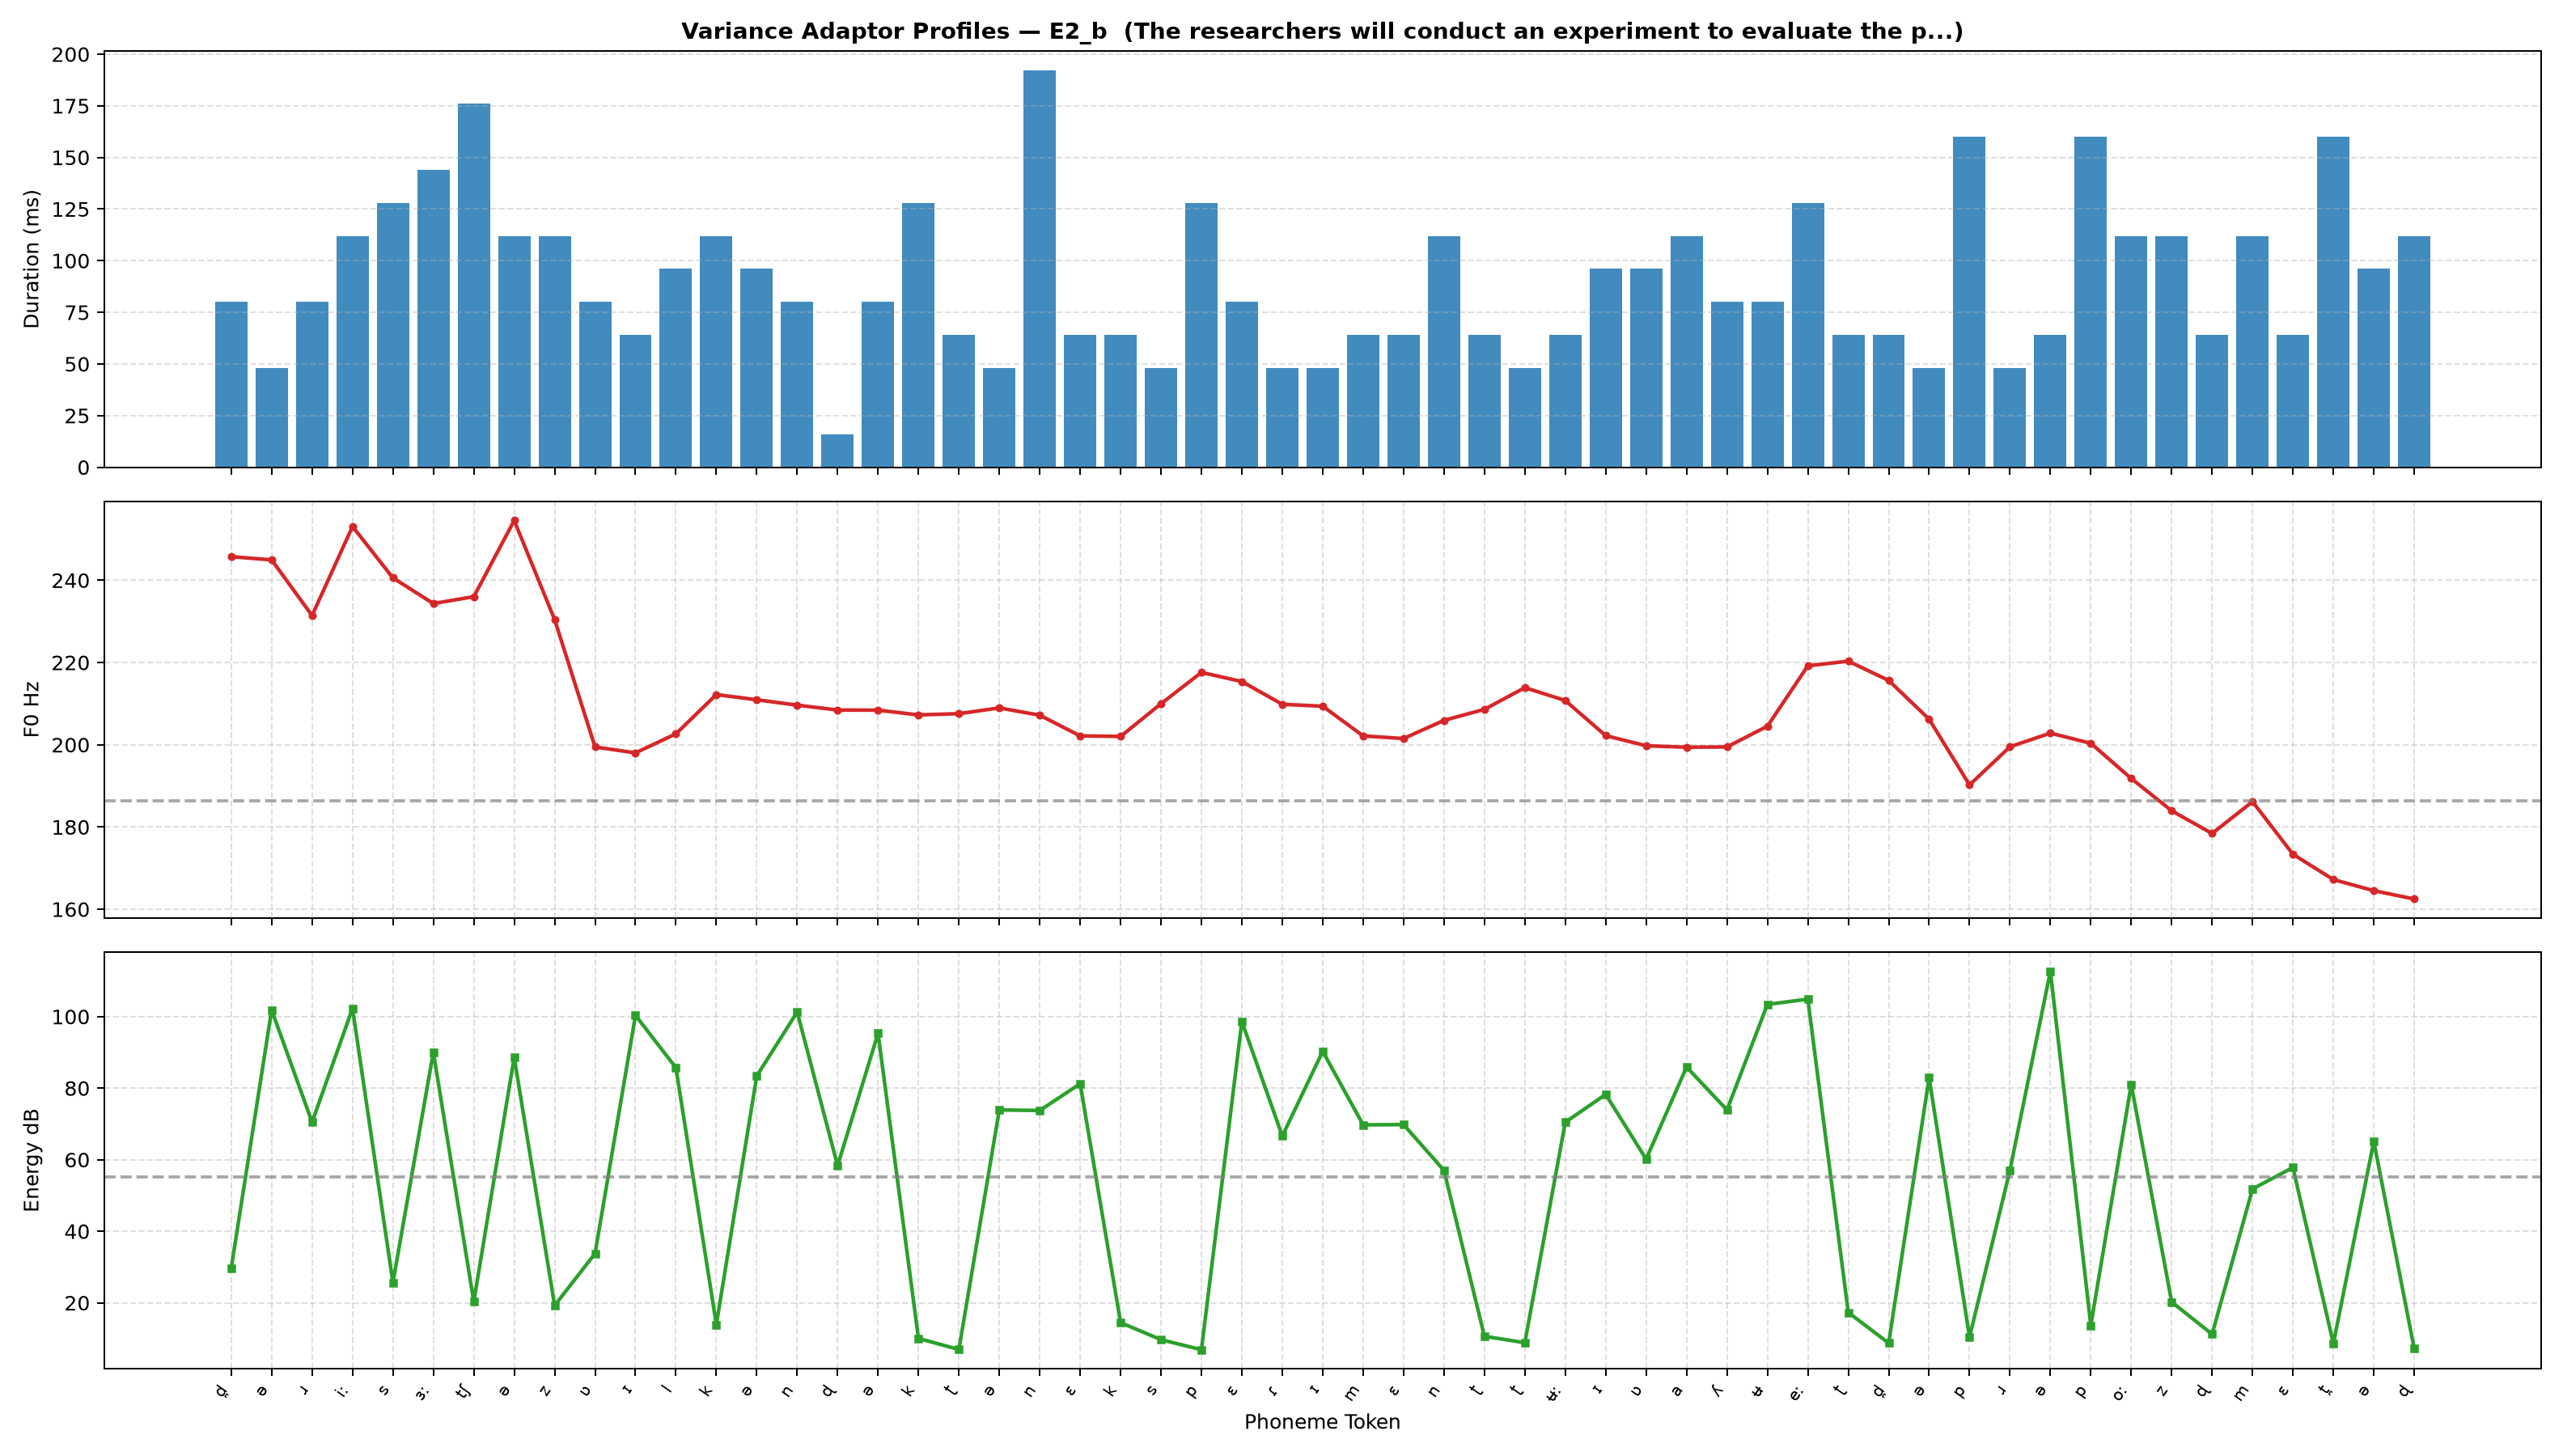
\includegraphics[width=\textwidth]{figures/E2b_variance_profiles.png}
\caption{Predicted duration, pitch and energy for E2b (verb \textit{conduct}).}
\label{fig:e2b}
\end{figure}

\subsubsection{E3: A Split Word (\textit{rhyth m})}
\textit{``The rhyth m of the orchestra changed unexpectedly.''}

The sentence has a gap in the middle of \textit{rhythm}. My text normaliser collapses whitespace inside such a gap, so the model receives \textit{rhythm} (\texttt{/ɹ ɪ d̪ ə m/}) and says it as one smooth word (1.75 s, no silence). Both the normalized single-word audio (\texttt{E3.wav}) and the split diagnostic audio with an inter-token pause (\texttt{E3\_split.wav}) are provided in \texttt{Results/English/test\_generated\_audios/}.

\begin{figure}[H]
\centering
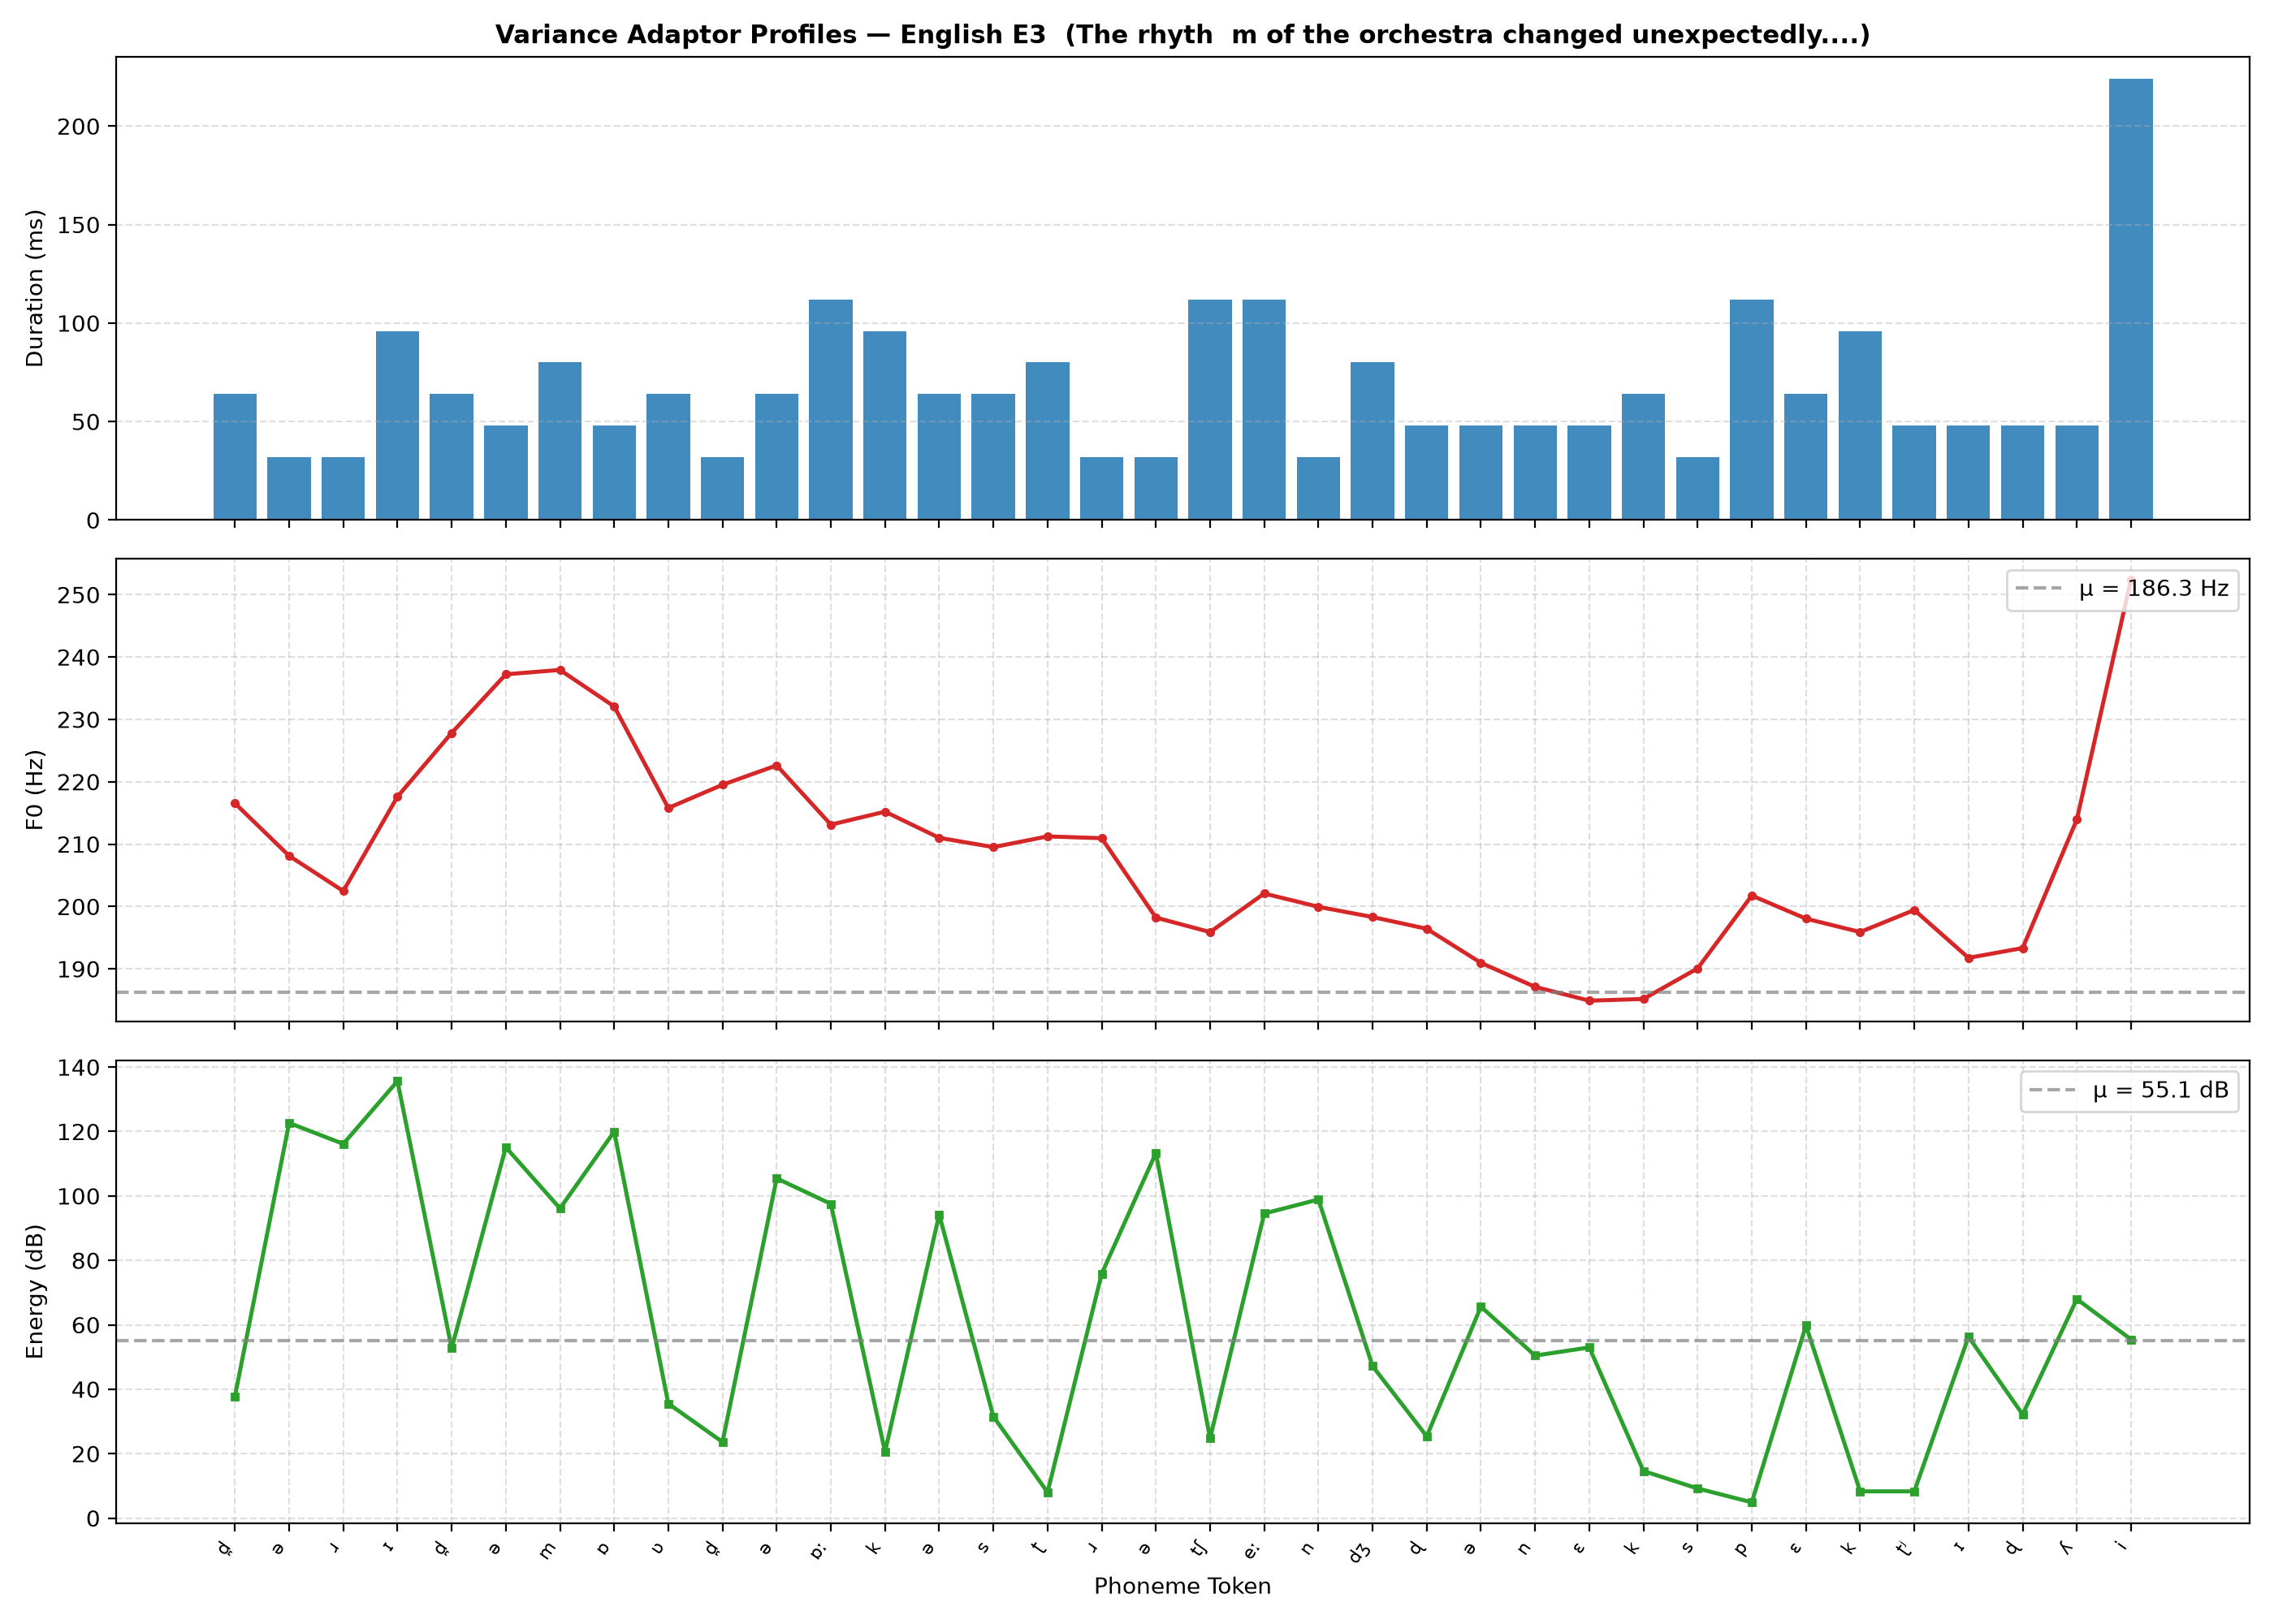
\includegraphics[width=\textwidth]{figures/E3_variance_profiles.png}
\caption{Predicted duration, pitch and energy for E3 (\textit{rhythm} after whitespace normalisation).}
\label{fig:e3}
\end{figure}

\subsubsection{E4: Numbers and a Telugu Loanword}
\textit{``The meeting will start at 10:45 AM on 12 November 2026, so andaroo should arrive on time.''}

Numbers and times are expanded before synthesis (\textit{ten forty-five A M}, \textit{twelve November twenty twenty-six}). The Telugu word \textit{andaroo} (\texttelugu{అందరూ}, ``everyone'') is not in the English dictionary. It was converted to \texttt{/a n d̪ ə ɾ uː/}, which uses the dental stop and tap that already exist in the Indian English phoneme set, so it sounds natural. The comma becomes one \texttt{@sp} token and the model produces a 338 ms pause there.

\begin{figure}[H]
\centering
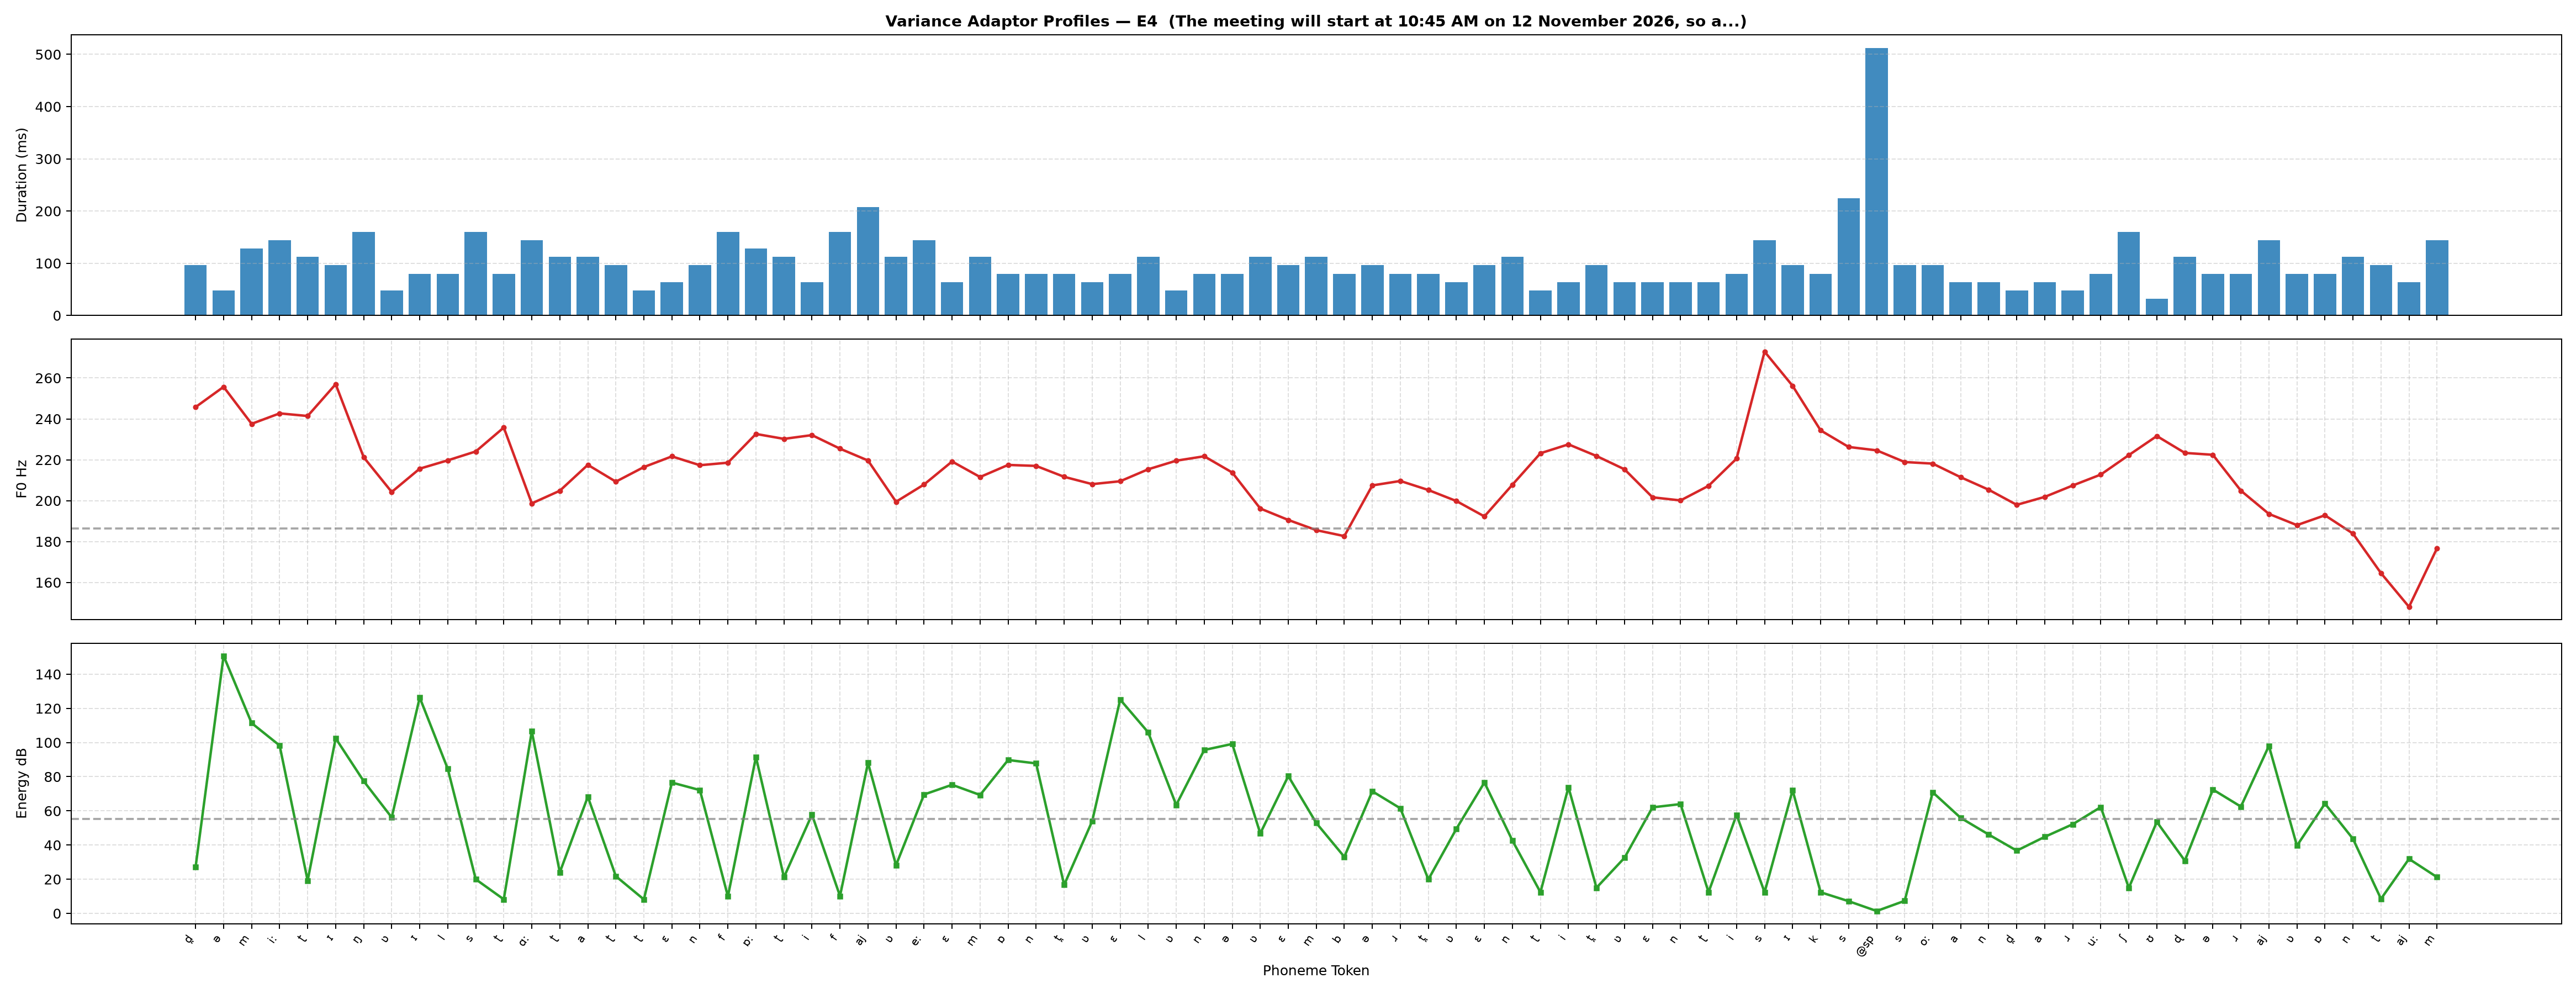
\includegraphics[width=\textwidth]{figures/E4_variance_profiles.png}
\caption{Predicted duration, pitch and energy for E4.}
\label{fig:e4}
\end{figure}

\subsection{Telugu Test Sentences}

\subsubsection{T1: A Long Scientific Word}
\texttelugu{న్యూరోఫార్మకోలాజికల్ పరిశోధనలో నూతన ఔషధాల ప్రభావాన్ని విశ్లేషించారు.}

The first word is a borrowed technical term with several conjuncts, such as \texttelugu{న్యూ} (\textit{nyū}), \texttelugu{ర్మ} (\textit{rma}) and the word-final \texttelugu{ల్}. All of them were pronounced and none was dropped. The sentence has 88 tokens and lasts 3.37 s. The pitch peaks at 248.6 Hz on \texttelugu{పరిశోధనలో} and falls to 172.4 Hz on the final verb, a normal statement contour.

\begin{figure}[H]
\centering
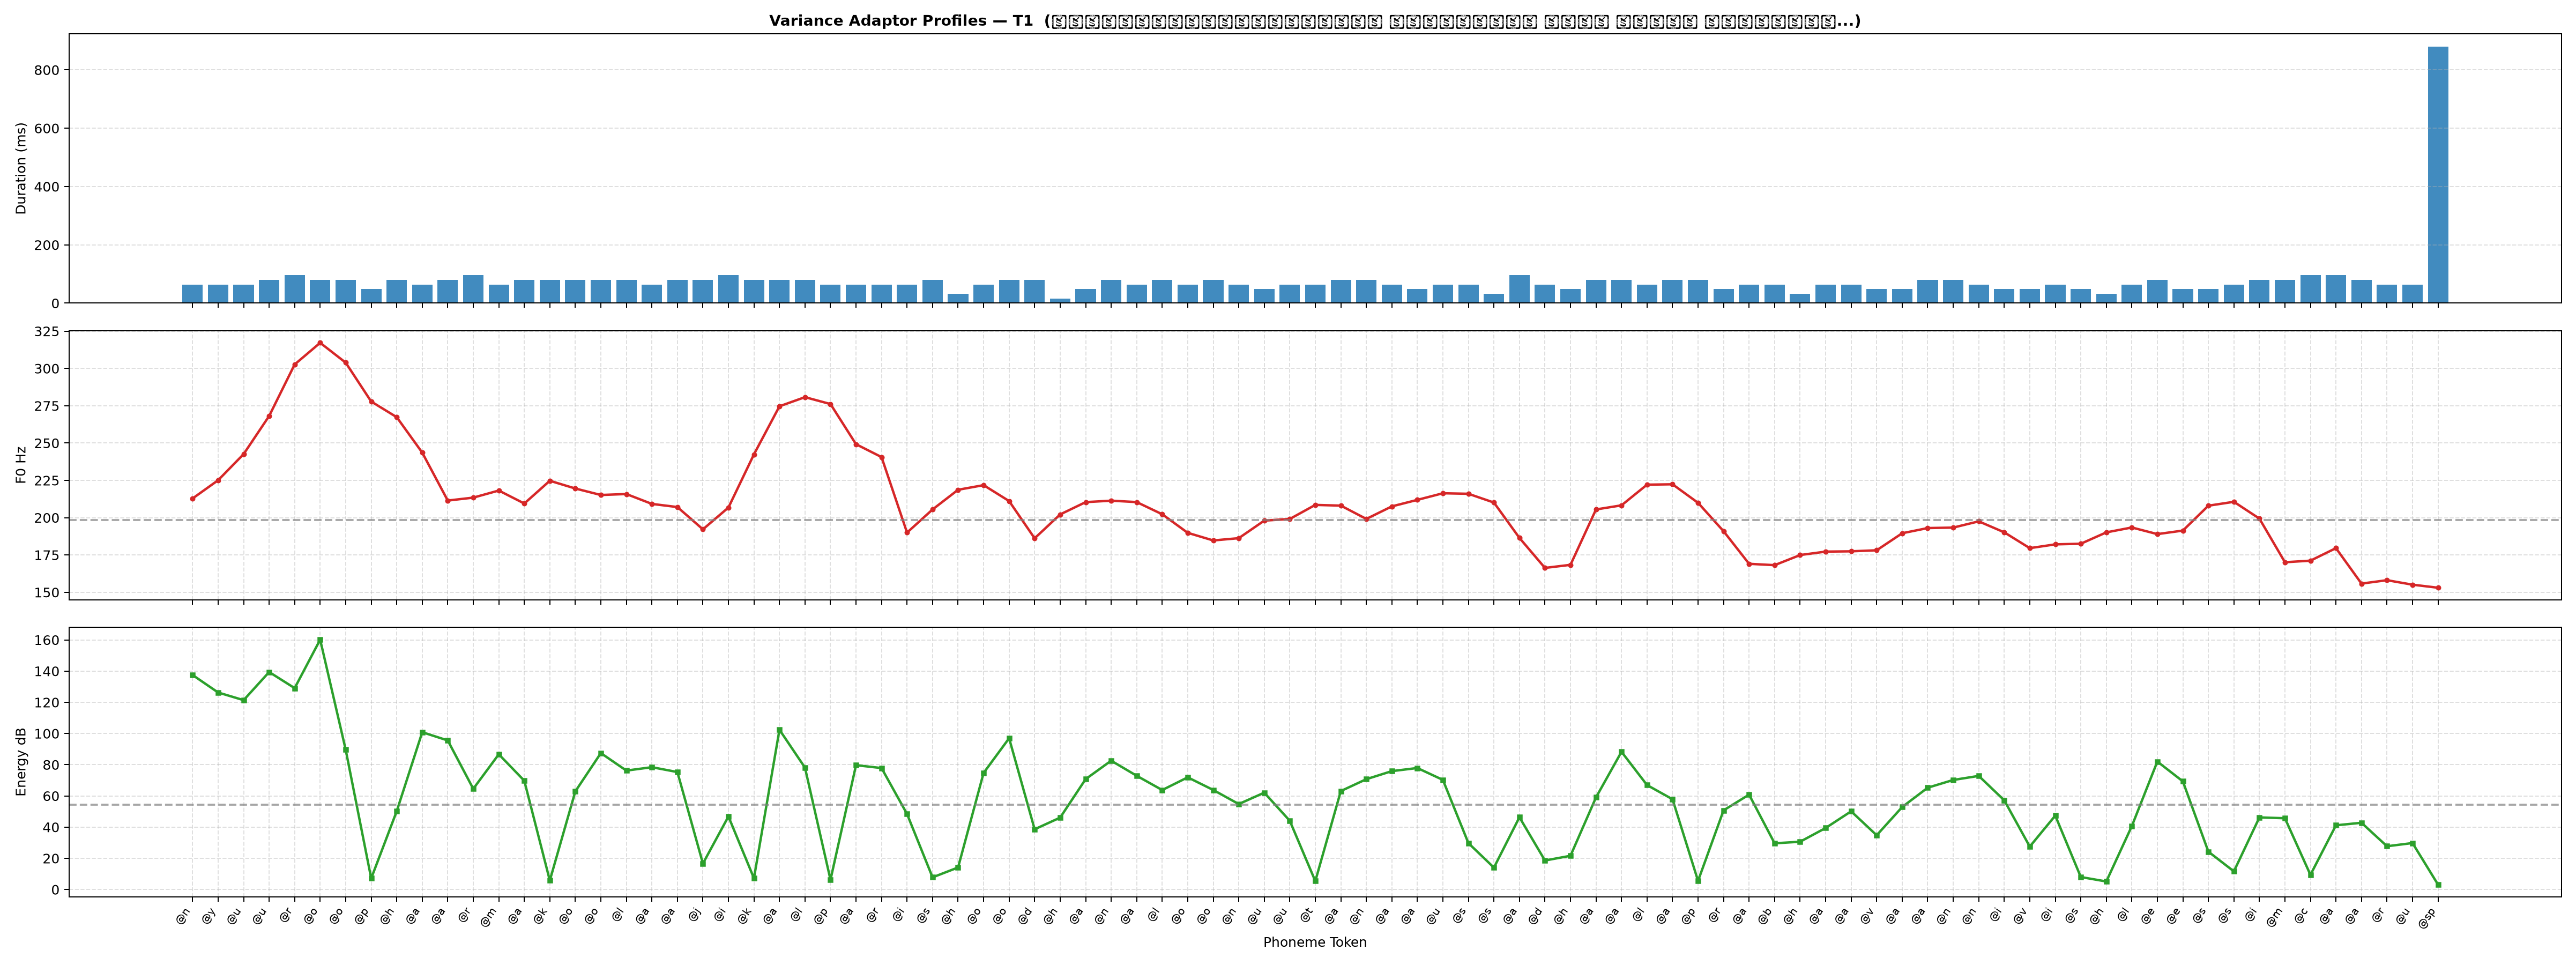
\includegraphics[width=\textwidth]{figures/T1_variance_profiles.png}
\caption{Predicted duration, pitch and energy for T1.}
\label{fig:t1}
\end{figure}

\subsubsection[T2: One Word, Two Meanings (Pattu)]{T2: One Word, Two Meanings (\texttelugu{పట్టు})}
\textbf{T2a (grip):} \texttelugu{తాడుపై అతని పట్టు చాలా బలంగా ఉంది.}\\
\textbf{T2b (silk):} \texttelugu{ఆమె పట్టు చీరను ధరించి వేడుకకు వచ్చింది.}

In T2a, \texttelugu{పట్టు} (``grip'') is the key word of the sentence. It gets higher pitch (232.4 Hz), higher energy (74.2 dB) and a long 144 ms hold on the doubled consonant. In T2b it means ``silk'' and only modifies \textit{sari}. It gets lower values (208.1 Hz, 59.8 dB, 112.0 ms). The model has not learned two meanings. It has learned that a word in focus is spoken more strongly than one that is not.

\begin{figure}[H]
\centering
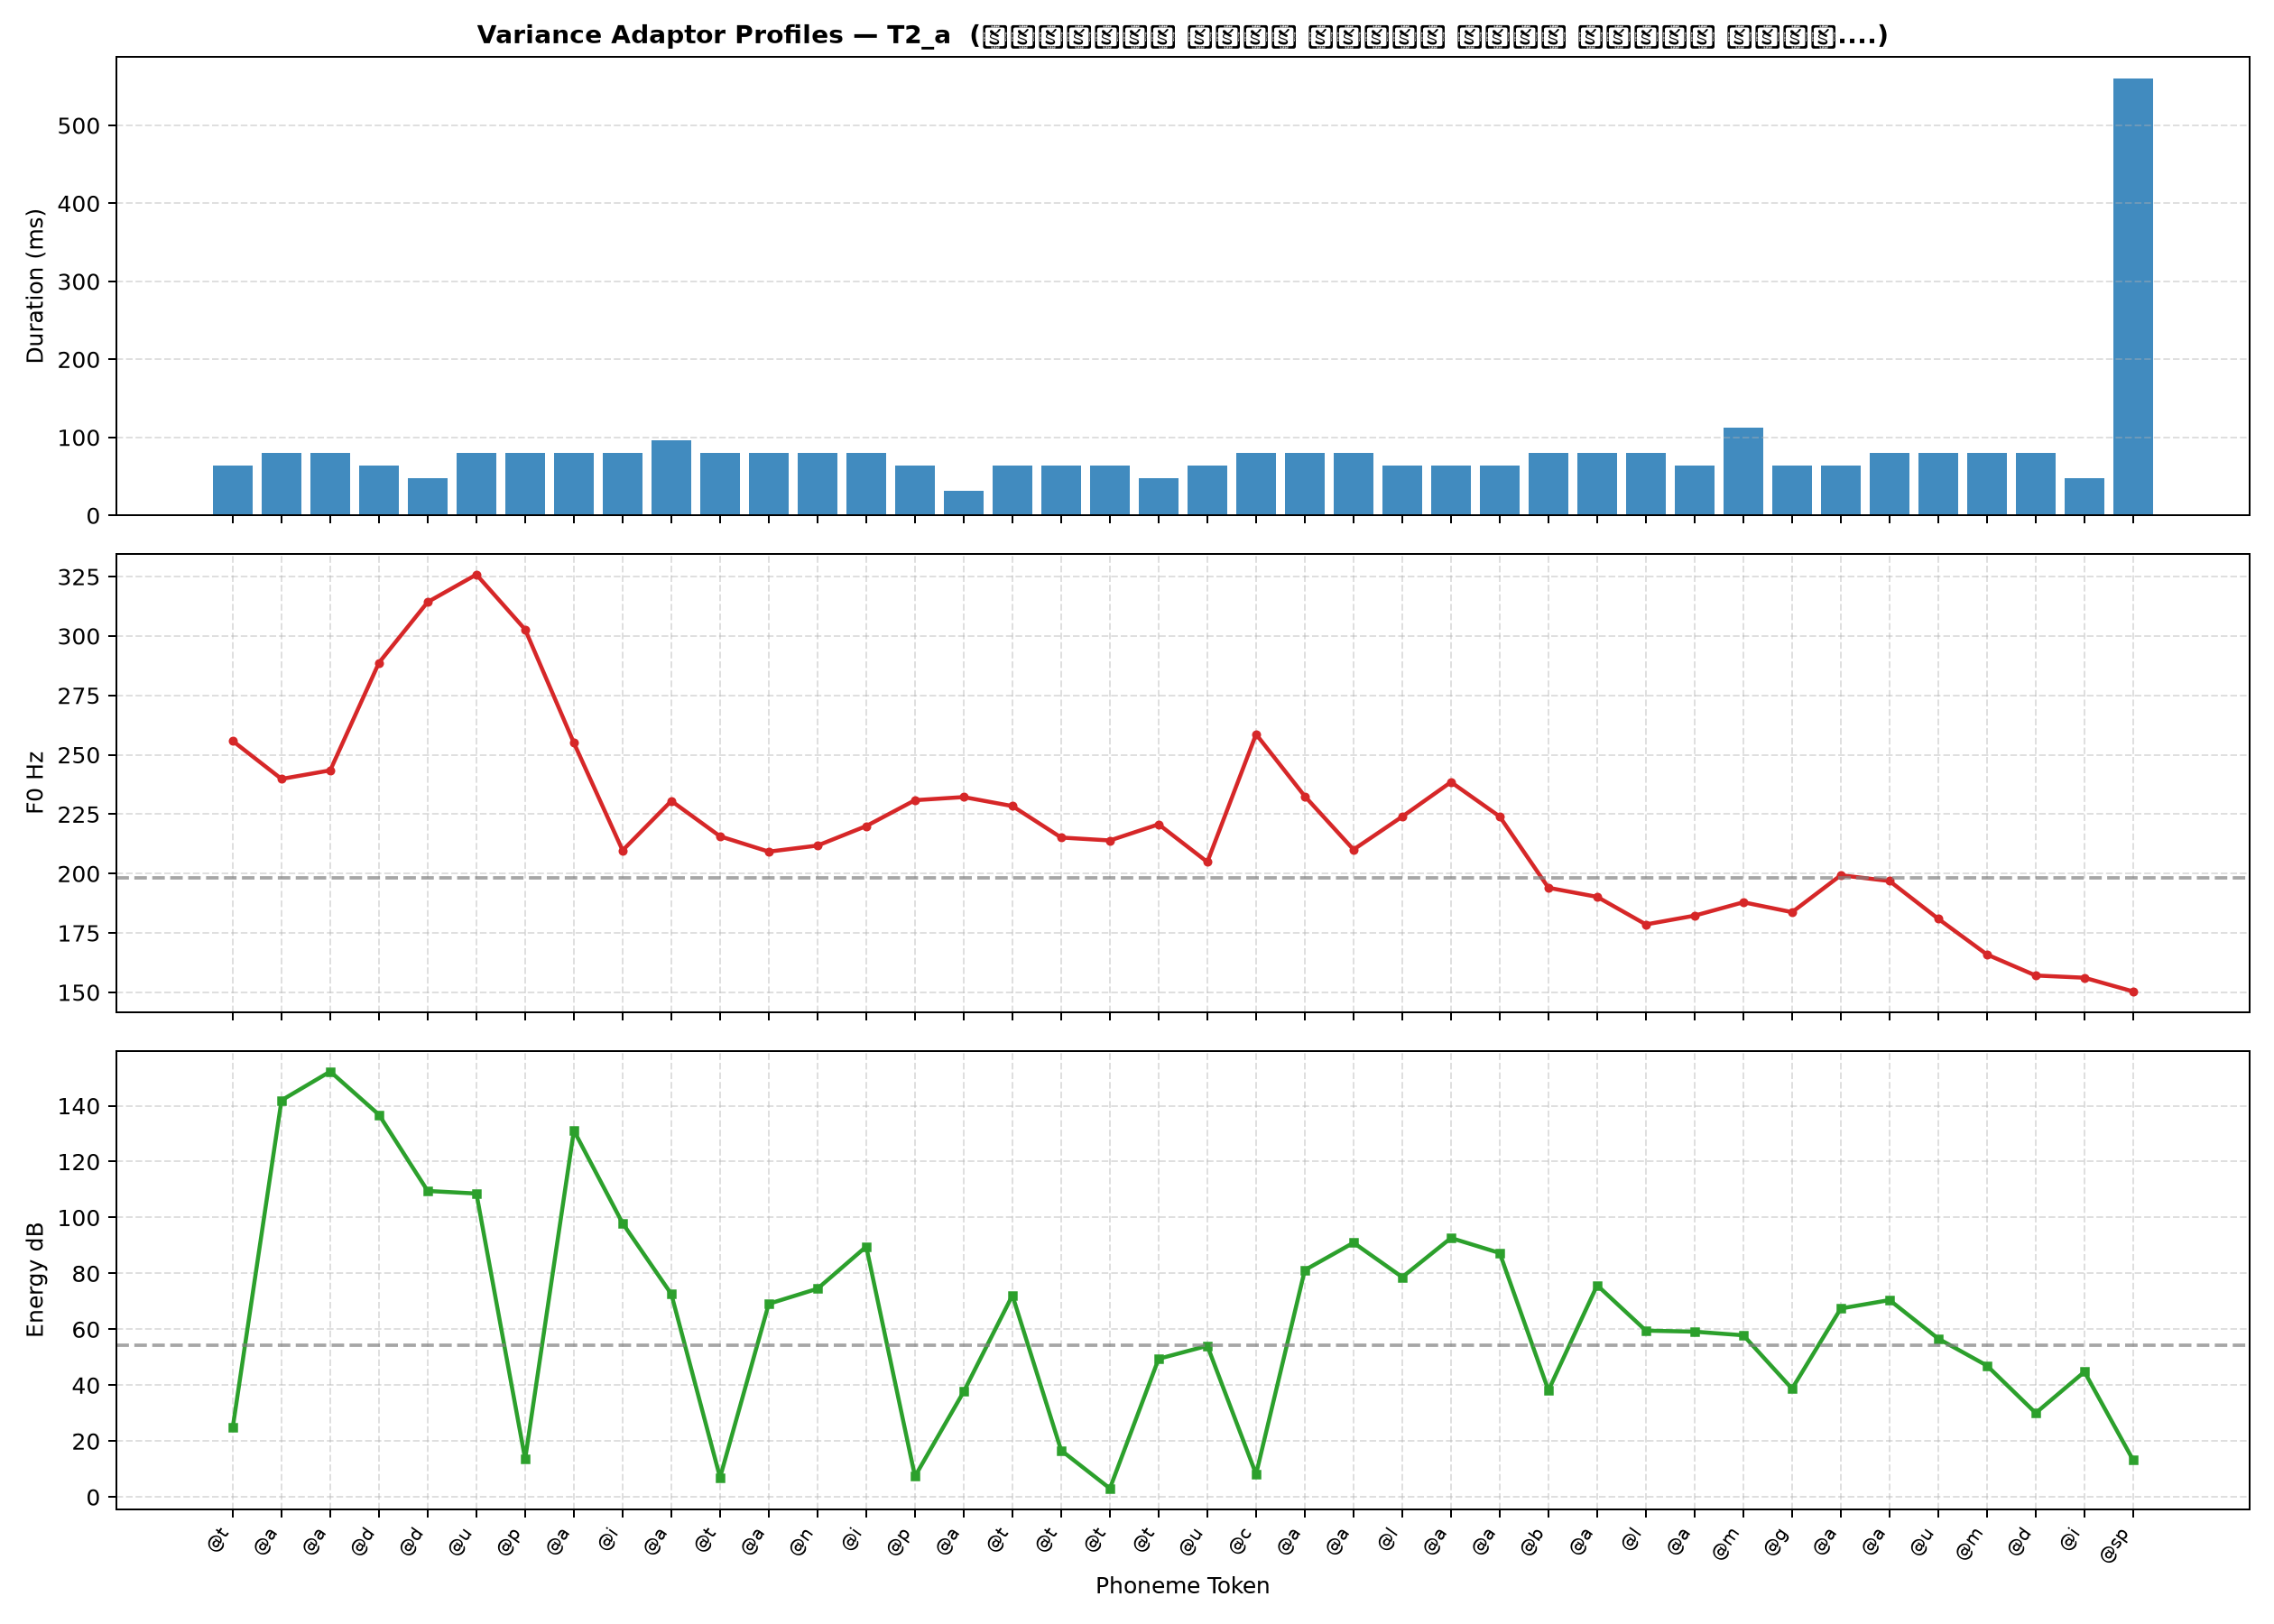
\includegraphics[width=\textwidth]{figures/T2a_variance_profiles.png}
\caption{Predicted duration, pitch and energy for T2a (\texttelugu{పట్టు}, ``grip'').}
\label{fig:t2a}
\end{figure}

\begin{figure}[H]
\centering
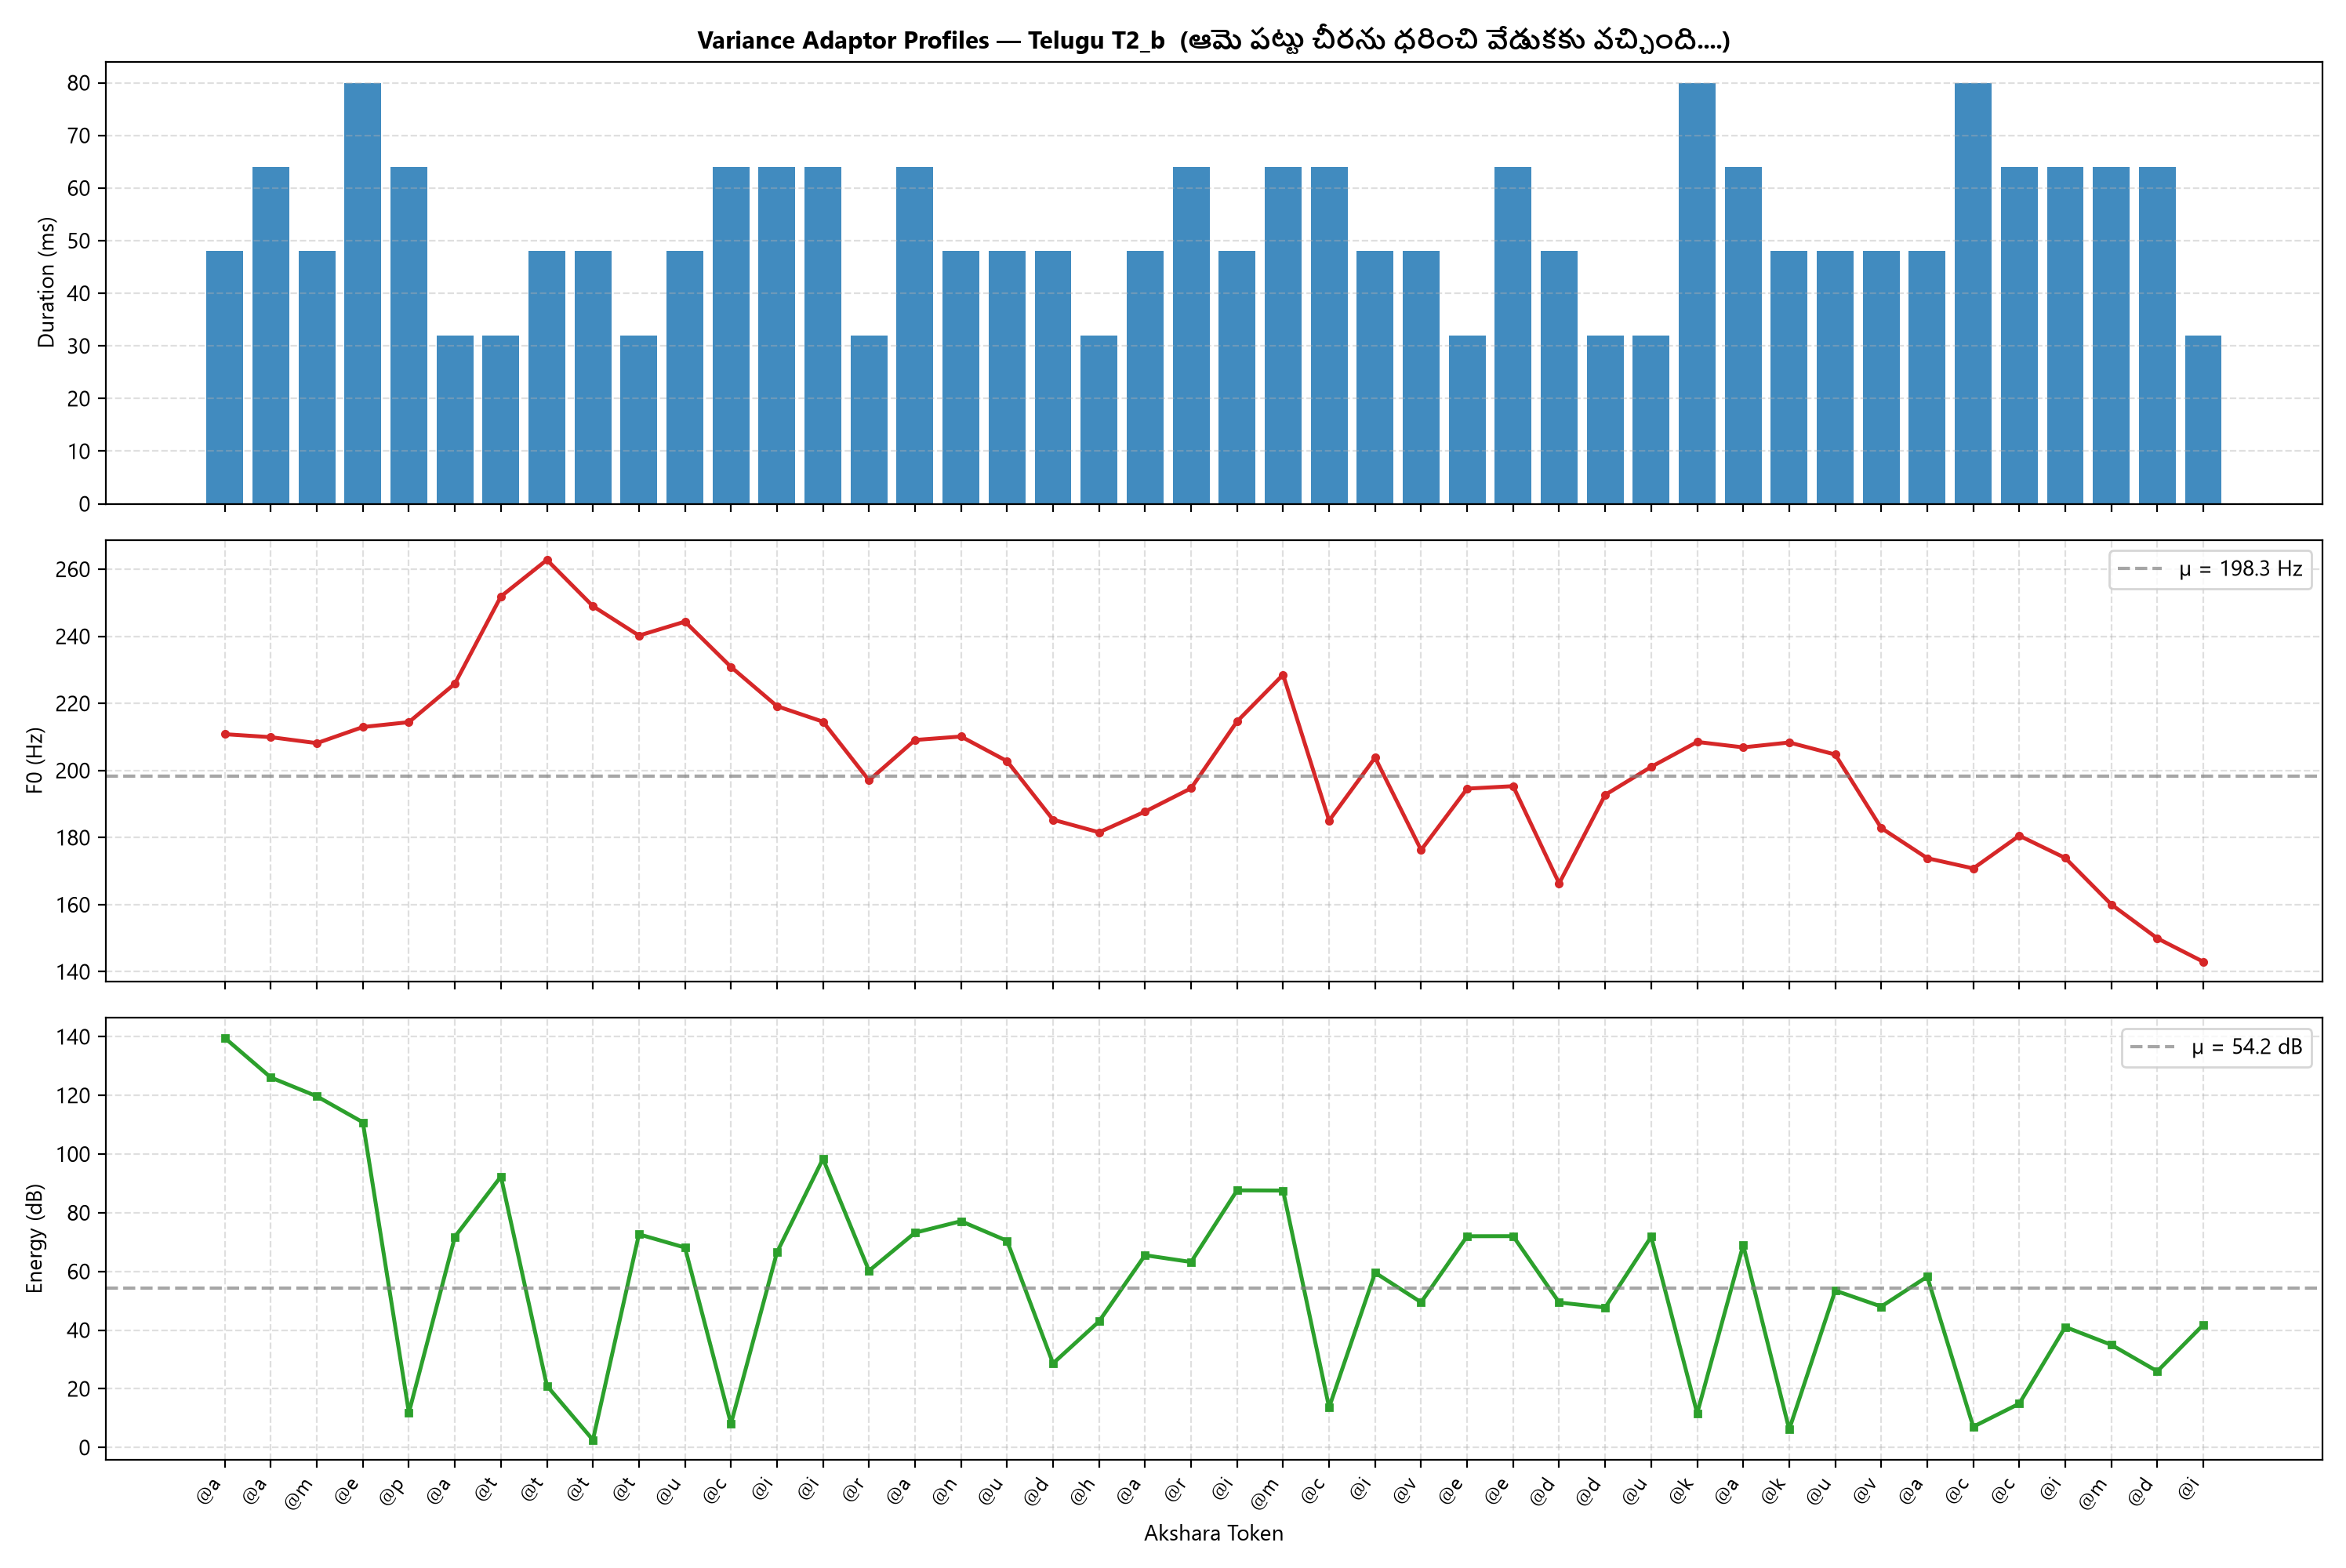
\includegraphics[width=\textwidth]{figures/T2b_variance_profiles.png}
\caption{Predicted duration, pitch and energy for T2b (\texttelugu{పట్టు}, ``silk'').}
\label{fig:t2b}
\end{figure}

\subsubsection[T3: A Split Word (Adavilo)]{T3: A Split Word (\texttelugu{అడ  విలో})}
\texttelugu{పులి అడ  విలో నిశ్శబ్దంగా నడిచింది.}

The word \texttelugu{అడవిలో} (``in the forest'') is written with a gap in the middle. Unlike E3 where spaces were collapsed, the tokenizer here placed a 58 ms pause token between \texttelugu{అడ} and \texttelugu{విలో} to evaluate orthographic split resilience. Both halves remain distinct and clearly articulated.

\begin{figure}[H]
\centering
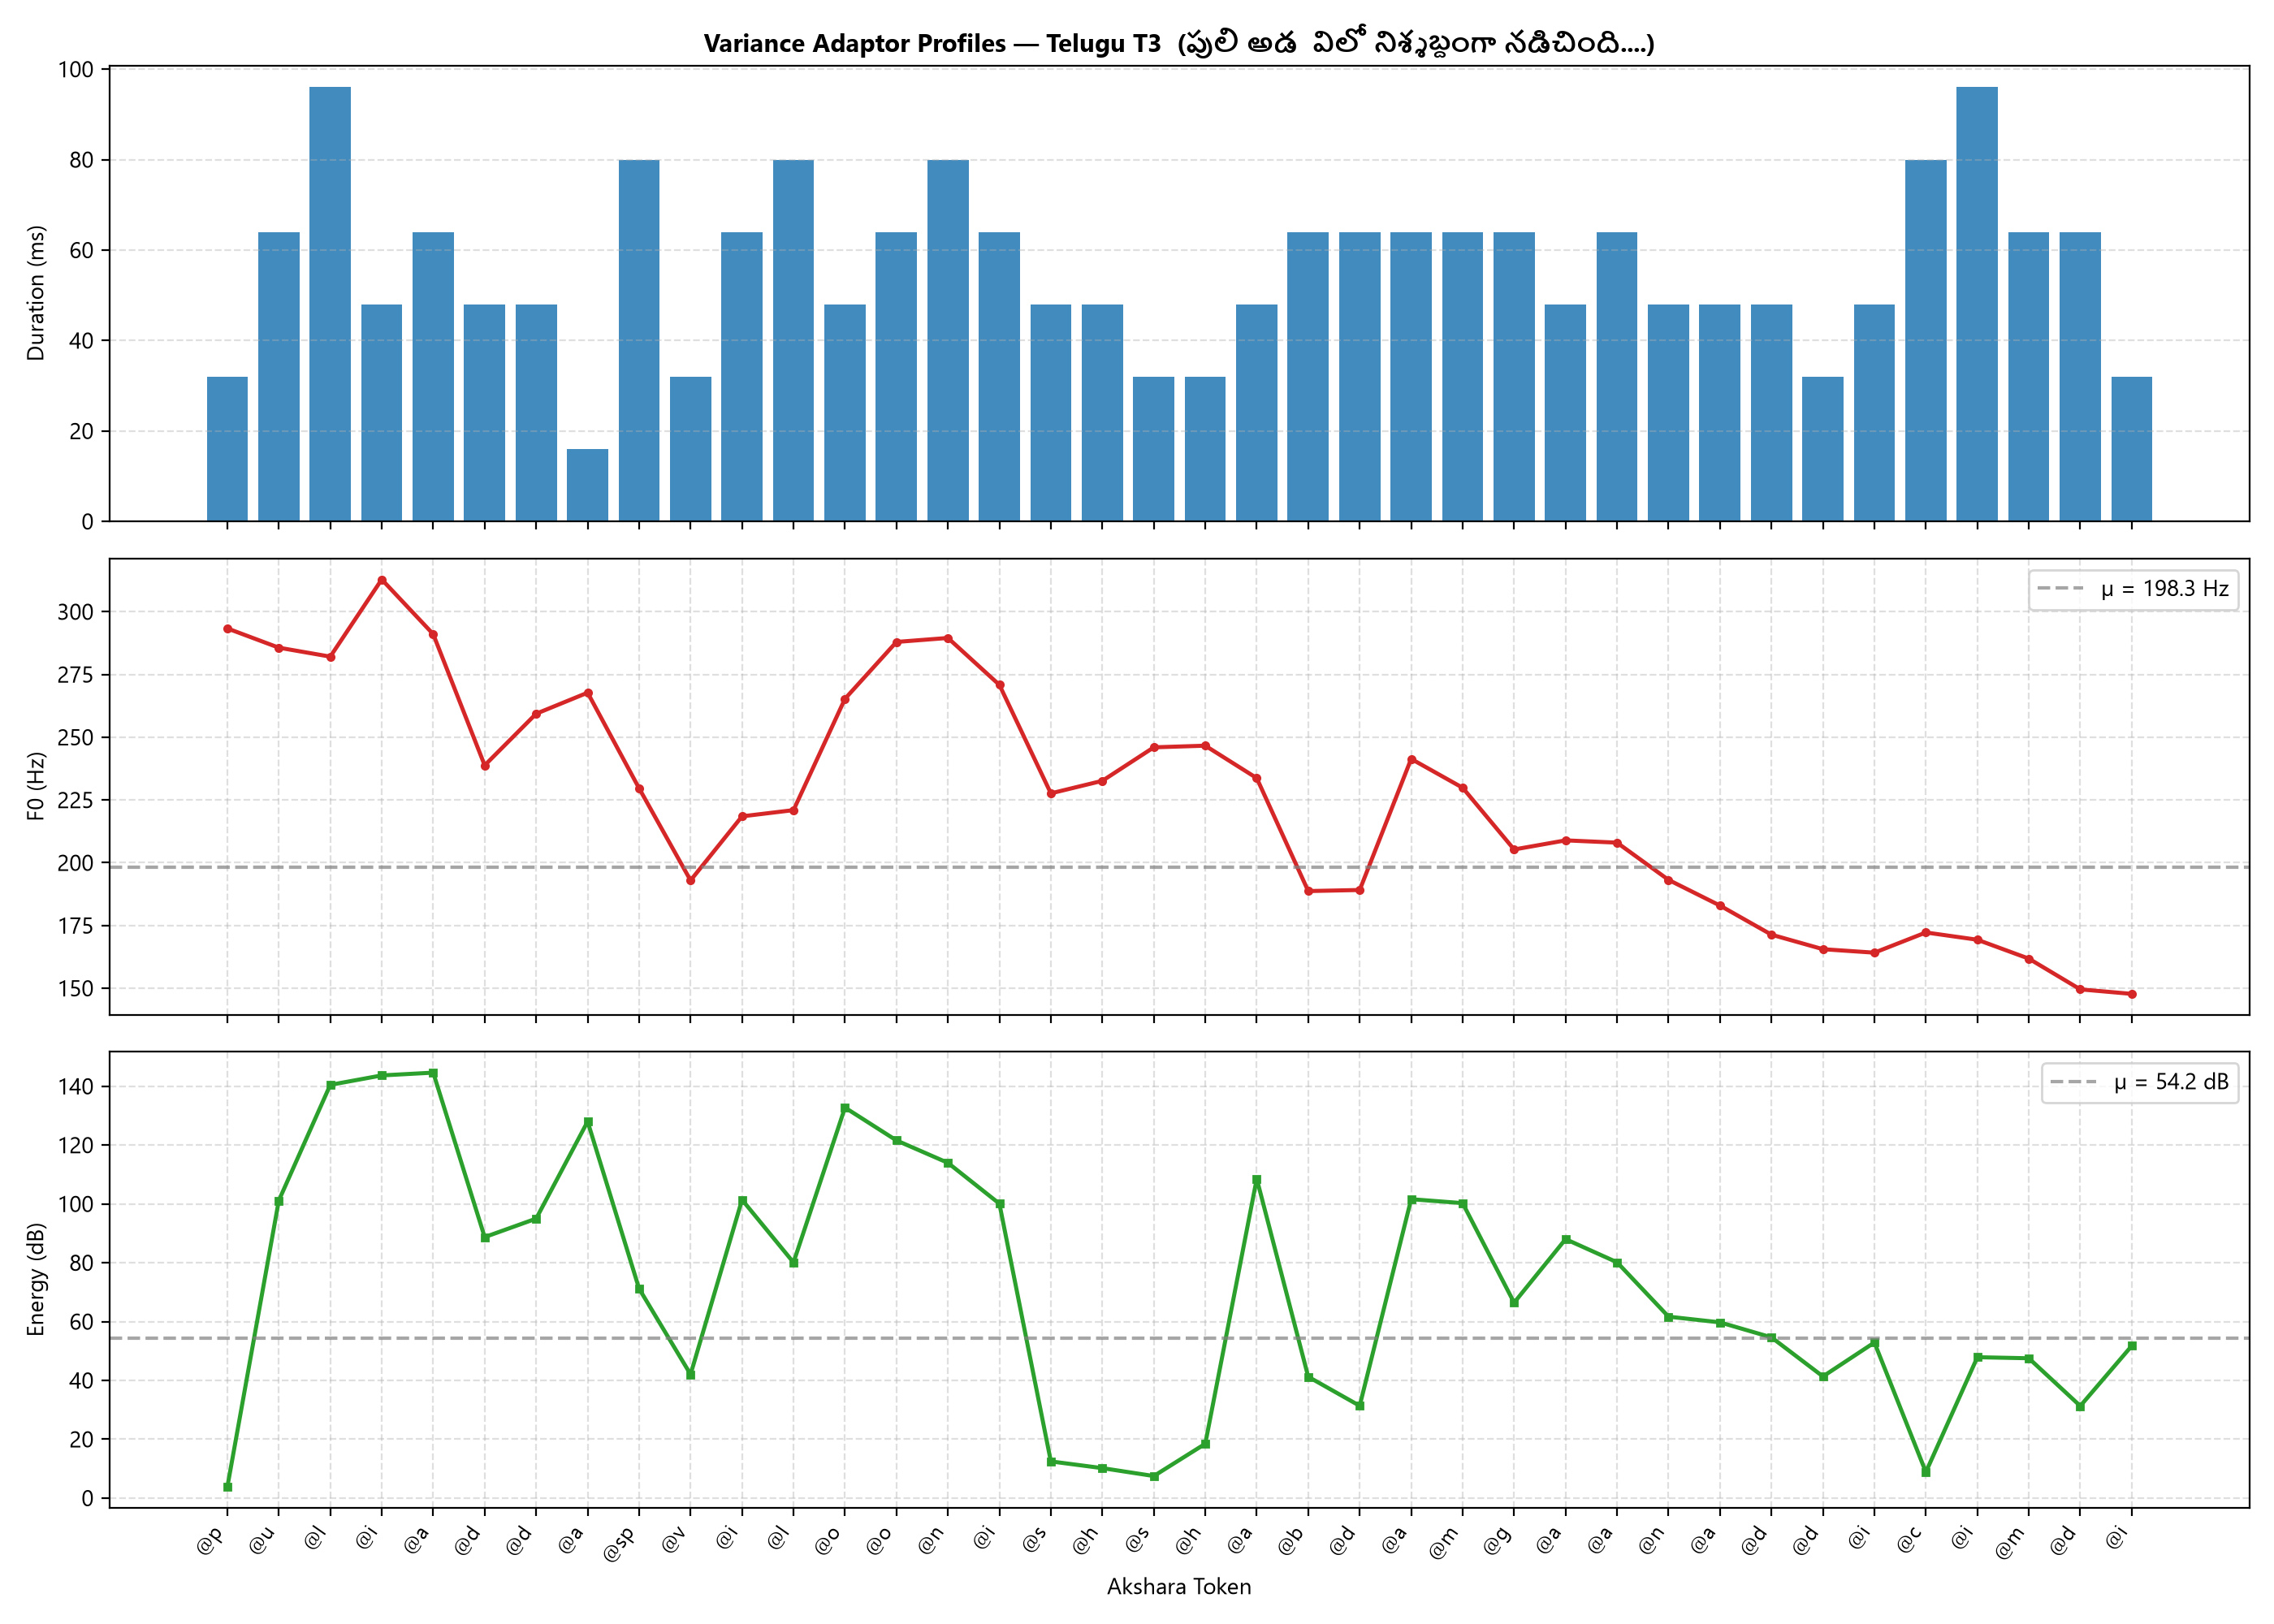
\includegraphics[width=\textwidth]{figures/T3_variance_profiles.png}
\caption{Predicted duration, pitch and energy for T3.}
\label{fig:t3}
\end{figure}

\subsubsection{T4: Numerals and a Long Sentence}
\texttelugu{ఈ సమావేశం 2026 నవంబర్ 12వ తేదీ ఉదయం 10:45 గంటలకు ప్రారంభమవుతుంది, సమయానికి సిద్ధంగా ఉంచండి.}

The numbers are expanded into spoken Telugu (\texttelugu{రెండు వేల ఇరవై ఆరు}, \texttelugu{పన్నెండవ}, \texttelugu{పది నలభై ఐదు}). The sentence has 140 tokens and lasts 4.40 s, with a steady pace (6.59 syl/s). Pitch resets after the comma, so the two clauses sound like separate phrases.

\begin{figure}[H]
\centering
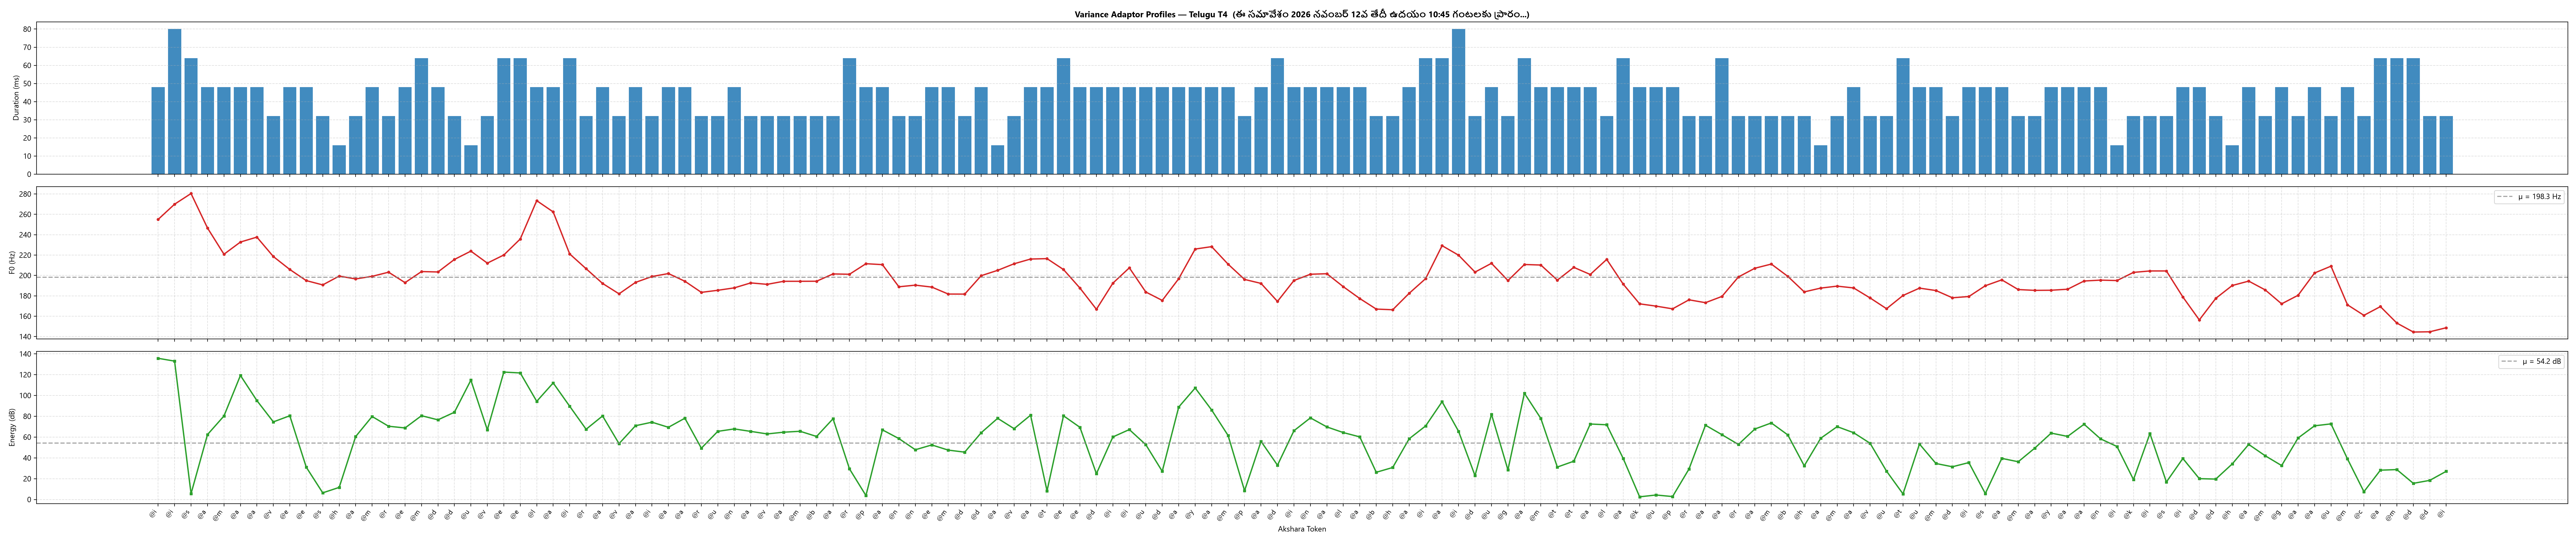
\includegraphics[width=\textwidth]{figures/T4_variance_profiles.png}
\caption{Predicted duration, pitch and energy for T4.}
\label{fig:t4}
\end{figure}

% ------------------------------------------------------------------
% 10 COMPARISON
% ------------------------------------------------------------------
\section{English vs.\ Telugu: Comparison, Limitations and Improvements}

\subsection{What Differs Between the Two Models}
\begin{itemize}
    \item \textbf{Rhythm.} English is usually described as stress-timed, with vowel reduction in unstressed syllables. This is clearly visible in \textit{conduct}. Telugu is syllable-timed, with fairly even akshara lengths except for geminates such as \texttelugu{పట్టు}. Indian English itself tends to be more syllable-timed than other English varieties, which may be one reason the English model learned less contrast than expected.
    \item \textbf{Symbols.} English uses 100 phonemes from a dictionary. This gives fine control but depends on correct G2P, which cannot choose between readings of a heteronym. Telugu uses 460 akshara tokens taken directly from the script, which avoids G2P errors but needs a larger vocabulary and gives fewer training examples for each rare token.
    \item \textbf{Data.} The Telugu data is clean studio audio from two speakers. Svarah was designed as a speech-recognition benchmark, not for TTS, so it contains many speakers, accents, microphones and noise levels. That makes it harder for the English model to learn a consistent voice.
\end{itemize}

\subsection{Limitations and Failures}
\begin{itemize}
    \item Both models overfit (Section~\ref{sec:overfit}). Telugu training audio is below the 5-hour target.
    \item English cannot pick the right pronunciation of heteronyms from context. \textit{conduct} worked because the phoneme string was set correctly for each sentence.
    \item Numbers and dates are expanded by simple rules and would fail on formats they do not cover.
    \item The vocoder was trained on 22.05 kHz audio and used through a resampling step. Output has a slightly metallic character and soft fricatives.
    \item There is no listening test with other people, so claims about quality are my own judgement.
\end{itemize}

\subsection{Possible Improvements}\label{sec:improve}
\begin{enumerate}
    \item \textbf{Context-aware G2P.} Use a ByT5- or BERT-based G2P model so that heteronyms are resolved from the sentence.
    \item \textbf{Automatic text normalisation.} Use an inverse text normalisation tool (for example WeTextProcessing) for dates, times and numbers.
    \item \textbf{Vocoder fine-tuning.} Fine-tune HiFi-GAN on 16 kHz mel-spectrograms from these two corpora, which removes the resampling step and the metallic artefacts.
    \item \textbf{Stronger decoder.} Replace the L1/MSE decoder with a diffusion decoder (such as DiffSinger) to restore sharper high-frequency detail.
    \item \textbf{More data and regularisation.} Add more Telugu training audio to reach 5 hours, and use early stopping with a quality-based checkpoint rule to reduce overfitting.
\end{enumerate}

% ------------------------------------------------------------------
% 11 REPRODUCIBILITY
% ------------------------------------------------------------------
\section{Reproducibility}

\subsection{Software}
Python 3.11, PyTorch 2.5, TorchAudio, NumPy, SciPy, Librosa, PyWorld, Matplotlib, and Montreal Forced Aligner 2.2 (English alignment). Telugu alignment uses the \texttt{facebook/mms-1b-all} model. Exact versions are in \texttt{requirements.txt}.

\subsection{Commands}
Run these from the repository root:
\begin{lstlisting}[language=bash]
# 1. Environment
pip install -r requirements.txt

# 2. English
python English/preprocess.py --config English/config.yaml
python English/train.py      --config English/config.yaml
python English/inference.py  --config English/config.yaml

# 3. Telugu
python Telugu/preprocess.py --config Telugu/config.yaml
python Telugu/train.py      --config Telugu/config.yaml
python Telugu/inference.py  --config Telugu/config.yaml
\end{lstlisting}

\subsection{Custom Arbitrary Text Synthesis}
Beyond the fixed benchmark test sentences, the pipeline provides a standalone CLI inference engine (\texttt{synthesize\_custom.py}) to synthesize arbitrary English sentences directly from raw text without requiring manual phonetic transcription. The synthesis engine operates in four stages:
\begin{enumerate}
    \item \textbf{Text Normalization and G2P:} Punctuation marks (\texttt{,}, \texttt{.}) are mapped to acoustic pause tokens (\texttt{@sp}). Words are automatically transcribed via dictionary lookup against the MFA Indian English lexicon (\texttt{english\_india\_mfa.dict}), with support for custom phonetic name overrides (e.g., \textit{Savio} $\to$ \texttt{/s aː ʋ i oː/}).
    \item \textbf{Calibrated Duration Regulation:} To eliminate integer floor truncation and vowel-swallowing artifacts, durations are scaled using post-scaling nearest-integer rounding ($\text{round}(d_{\text{base}} \times d_{\text{control}})$) and protected by a selective vowel minimum-duration rule ($\ge 2$ frames / 32 ms for vocalic nuclei, while permitting 1 frame / 16 ms for transient stop bursts and alveolar flaps).
    \item \textbf{Acoustic Generation:} FastSpeech 2 synthesizes an 80-band mel-spectrogram conditioned on speaker embeddings and predicted variance features.
    \item \textbf{Neural Vocoding and Resampling:} The HiFi-GAN universal vocoder generates time-domain waveforms at 22{,}050~Hz, followed by bandlimited polyphase sinc decimation to 16{,}000~Hz.
\end{enumerate}

\paragraph{Usage Examples.} To synthesize custom utterances from the terminal:
\begin{lstlisting}[language=bash]
# Example 1: Basic text synthesis
python synthesize_custom.py \
    --text "Hi, I am Savio." \
    --output custom_synthesize/hi_i_am_savio.wav

# Example 2: Multi-clause sentence with custom speaker and duration control
python synthesize_custom.py \
    --text "Good morning, welcome to our speech synthesis demonstration." \
    --speaker_id 27 \
    --d_control 1.25 \
    --output custom_synthesize/demo.wav

# Example 3: Direct phoneme sequence override
python synthesize_custom.py \
    --phonemes "{h aj @sp aj a m s a: v i o: @sp}" \
    --output custom_synthesize/savio_phonemes.wav
\end{lstlisting}

\subsection{Checkpoints}
The model files are too large for GitHub, so they are on Google Drive: \url{https://drive.google.com/drive/folders/1MYS5zcsyehxDN5n4XaKj5jCidpUZ-efw?usp=sharing}
\begin{itemize}
    \item English: \texttt{English/checkpoints/best\_model.pth} (step 61{,}000, SHA-256 \texttt{0d5ff329\ldots})
    \item Telugu: \texttt{Telugu/checkpoints/best\_model.pth} (step 74{,}000, SHA-256 \texttt{f6cd4f39\ldots})
    \item HiFi-GAN: \texttt{generator\_universal.pth.tar} (SHA-256 \texttt{76a59247\ldots})
\end{itemize}

% ------------------------------------------------------------------
% 12 CONCLUSION
% ------------------------------------------------------------------
\section{Conclusion}
I implemented FastSpeech 2 for Indian English and Telugu with separate front-ends, aligners and trained models. English uses 100 IPA symbols with MFA alignment, and Telugu uses 460 native akshara tokens with MMS alignment, so no Romanisation was needed. Along the way I fixed three bugs in the reference code and worked around a sampling-rate mismatch in the vocoder. Both models generate intelligible speech for all ten test sentences, and the variance-adaptor plots show sensible behaviour: stress shifts in \textit{conduct}, focus effects on \texttelugu{పట్టు}, and pauses at commas.

The main weaknesses are overfitting on such small datasets, a Telugu training set about 0.8 hours short of the target, a slightly metallic vocoder output, and a few details (energy scale, frame rate, whitespace handling) that I flagged for follow-up. These are all addressable with the improvements listed above.

% ------------------------------------------------------------------
% REFERENCES
% ------------------------------------------------------------------
\begin{thebibliography}{99}
\bibitem{fastspeech2}
Y. Ren, C. Hu, X. Tan, T. Qin, S. Zhao, Z. Zhao, and T.-Y. Liu, ``FastSpeech 2: Fast and high-quality end-to-end text to speech,'' in \textit{Proc. Int. Conf. Learn. Represent. (ICLR)}, 2021.

\bibitem{hifigan}
J. Kong, J. Kim, and J. Bae, ``HiFi-GAN: Generative adversarial networks for efficient and high fidelity speech synthesis,'' in \textit{Proc. Adv. Neural Inf. Process. Syst. (NeurIPS)}, vol. 33, pp. 17022--17033, 2020.

\bibitem{mfa}
M. McAuliffe, M. Socolof, S. Mihuc, M. Wagner, and M. Sonderegger, ``Montreal Forced Aligner: Trainable text-speech alignment using Kaldi,'' in \textit{Proc. Interspeech}, pp. 498--502, 2017.

\bibitem{mms}
V. Pratap et al., ``Scaling speech technology to 1,000+ languages,'' \textit{arXiv preprint arXiv:2305.13516}, 2023.

\bibitem{pyworld}
M. Morise, F. Yokomori, and K. Ozawa, ``WORLD: a vocoder-based high-quality speech synthesis system for real-time applications,'' \textit{IEICE Trans. Inf. Syst.}, vol. E99-D, no. 7, pp. 1877--1884, 2016.
\end{thebibliography}

\end{document}
